%%%%%%%%%%%%%%%%%%%%%%%%%%%%%%%%%%%%%%%%%%%%%%%%%%%%%%%%%%%%%%%%%%%%%%%%%%%%%%%%
%% Plantilla de memoria en LaTeX para la ETSIT - Universidad Rey Juan Carlos
%%
%% Por Gregorio Robles <grex arroba gsyc.urjc.es>
%%     Grupo de Sistemas y Comunicaciones
%%     Escuela Técnica Superior de Ingenieros de Telecomunicación
%%     Universidad Rey Juan Carlos
%% (muchas ideas tomadas de Internet, colegas del GSyC, antiguos alumnos...
%%  etc. Muchas gracias a todos)
%%
%% La última versión de esta plantilla está siempre disponible en:
%%     https://github.com/gregoriorobles/plantilla-memoria
%%
%% Para obtener PDF, ejecuta en la shell:
%%   make
%% (las imágenes deben ir en PNG o JPG)

%%%%%%%%%%%%%%%%%%%%%%%%%%%%%%%%%%%%%%%%%%%%%%%%%%%%%%%%%%%%%%%%%%%%%%%%%%%%%%%%

\documentclass[a4paper, 12pt]{book}
%\usepackage[T1]{fontenc}

\usepackage[a4paper, left=2.5cm, right=2.5cm, top=3cm, bottom=3cm]{geometry}
\usepackage{times}
\usepackage[utf8]{inputenc}
\usepackage[spanish]{babel} % Comenta esta línea si tu memoria es en inglés
\usepackage{url}
%\usepackage[dvipdfm]{graphicx}
\usepackage{graphicx}
\usepackage{float}  %% H para posicionar figuras
\usepackage[nottoc, notlot, notlof, notindex]{tocbibind} %% Opciones de índice
\usepackage{latexsym}  %% Logo LaTeX

\title{Memoria del Proyecto}
\author{Nombre del autor}

\renewcommand{\baselinestretch}{1.5}  %% Interlineado

\begin{document}

\renewcommand{\refname}{Bibliografía}  %% Renombrando

%%%%%%%%%%%%%%%%%%%%%%%%%%%%%%%%%%%%%%%%%%%%%%%%%%%%%%%%%%%%%%%%%%%%%%%%%%%%%%%%
% PORTADA

\begin{titlepage}
\begin{center}

\includegraphics[scale=0.8]{img/URJ_logo_Color_POS.png}

\vspace{1.75cm}

\Large
GRADO EN INGENIERIA EN SISTEMAS AUDIOVISUALES Y MULTIMEDIA 

\vspace{0.4cm}

\large
Curso Académico 2020/2021

\vspace{0.8cm}

Trabajo Fin de Grado

\vspace{2.5cm}

\LARGE
SIMULADOR DE TRAZAS DE COMUNICACIONES EN REALIDAD VIRTUAL

\vspace{4cm}

\large
Autor : Alejandro Esteban López \\
Tutor : Dr. Jesus María González Barahona
\end{center}
\end{titlepage}

\newpage
\mbox{}
\thispagestyle{empty} % para que no se numere esta pagina


%%%%%%%%%%%%%%%%%%%%%%%%%%%%%%%%%%%%%%%%%%%%%%%%%%%%%%%%%%%%%%%%%%%%%%%%%%%%%%%%
%%%% Para firmar
\clearpage
\pagenumbering{gobble}
\chapter*{}

\vspace{-4cm}
\begin{center}
\LARGE
\textbf{Trabajo Fin de Grado}

\vspace{1cm}
\large
Simulador de Trazas de Comunicaciones en Realidad Virtual

\vspace{1cm}
\large
\textbf{Autor :} Alejandro Esteban López \\
\textbf{Tutor :} Dr. Jesus María González Barahona

\end{center}

\vspace{1cm}
La defensa del presente Proyecto Fin de Carrera se realizó el día \qquad$\;\,$ de \qquad\qquad\qquad\qquad \newline de 202X, siendo calificada por el siguiente tribunal:


\vspace{0.5cm}
\textbf{Presidente:}

\vspace{1.2cm}
\textbf{Secretario:}

\vspace{1.2cm}
\textbf{Vocal:}


\vspace{1.2cm}
y habiendo obtenido la siguiente calificación:

\vspace{1cm}
\textbf{Calificación:}


\vspace{1cm}
\begin{flushright}
\label{sec:Github}
\end{flushright}

%%%%%%%%%%%%%%%%%%%%%%%%%%%%%%%%%%%%%%%%%%%%%%%%%%%%%%%%%%%%%%%%%%%%%%%%%%%%%%%%
%%%% Dedicatoria

\chapter*{}
\pagenumbering{Roman} % para comenzar la numeracion de paginas en numeros romanos
\begin{flushright}
\textit{Dedicado a \\
mis padres.}
\end{flushright}

%%%%%%%%%%%%%%%%%%%%%%%%%%%%%%%%%%%%%%%%%%%%%%%%%%%%%%%%%%%%%%%%%%%%%%%%%%%%%%%%
%%%% Agradecimientos

\chapter*{Agradecimientos}
%\addcontentsline{toc}{chapter}{Agradecimientos} % si queremos que aparezca en el índice
\markboth{AGRADECIMIENTOS}{AGRADECIMIENTOS} % encabezado 

En primer lugar quería dar las gracias a mis padres, ya que sin ellos nada de esto hubiera sido posible. Ellos han dedicado todo su tiempo, su esfuerzo y sus recursos con tal de educarme y formarme lo mejor posible para afrontar la vida. Siempre me han ayudado en todo, incluso cuando he estado a punto de tirar la toalla y dejarlo, ellos estaban ahí para darme el empujón necesario y la motivación para seguir con ello y finalmente poder conseguirlo. Gracias, gracias y gracias de corazón, por todo lo que habéis hecho y hacéis por mí, nunca estaré lo suficientemente agradecido de todo lo que me habéis dado y enseñado. Os quiero mucho.

Darle las gracias a mi hermano, que aunque a veces tengamos nuestros más y nuestros menos, siempre está ahí para todo lo que necesito ayudándome y dándome los mejores consejos posibles siempre que los necesito.

También quería darle las gracias a mi pareja, que siempre está ahí apoyándome tanto en los buenos momentos como sobre todo en los malos momentos, con todo lo que ello conlleva. Siempre me saca una sonrisa y me hace sentir especial a su lado.

Y por último agradecer a mi tutor Jesús M. González Barahona que desde el principio siempre ha tenido disponibilidad para resolverme cualquier duda y ayudarme en cualquier cosa que necesitase.
%%%%%%%%%%%%%%%%%%%%%%%%%%%%%%%%%%%%%%%%%%%%%%%%%%%%%%%%%%%%%%%%%%%%%%%%%%%%%%%%
%%%% Resumen

\chapter*{Resumen}
%\addcontentsline{toc}{chapter}{Resumen} % si queremos que aparezca en el índice
\markboth{RESUMEN}{RESUMEN} % encabezado

El proyecto está construido para interpretar capturas realizadas por el programa Wireshark. Su función es la de leer la captura introducida e interpretar los campos que nos interesan, para poder representar, en una escena de Realidad Virtual en 3D, como es la red que se compone a través de las trazas obtenidas.

En la escena, podremos ver todos los nodos que hay en la red, tanto en la capa Ethernet como IP, con sus correspondientes carteles identificando que IP o dirección Ethernet tienen.
Estos nodos estarán conectados entre sí, solamente entre los que se intercambien paquetes.

Los paquetes podremos verlos también representados y en una animación, en la que veremos como se desplazan desde su nodo origen hasta su nodo destino. Dentro de cada paquete, al pinchar sobre él, podremos también ver las capas que tiene ese paquete, y los datos más relevantes de cada una de ellas, que se representaran en un cartel encima de ellos.

El proyecto está basado en tecnología A-Frame, un framework de JavaScript, el cual se utiliza para la creación de escenas en realidad virtual. Para ello he construido el código mediante HTML5 y JavaScript.

También he ido incluyendo en un repositorio de GitHub todas las pruebas y avances que he ido realizando durante el proceso de elaboración del proyecto, para tener sincronizado y actualizado a la última versión el código final.

%%%%%%%%%%%%%%%%%%%%%%%%%%%%%%%%%%%%%%%%%%%%%%%%%%%%%%%%%%%%%%%%%%%%%%%%%%%%%%%%
%%%% Resumen en inglés

\chapter*{Summary}
%\addcontentsline{toc}{chapter}{Summary} % si queremos que aparezca en el índice
\markboth{SUMMARY}{SUMMARY} % encabezado

The project is built to interpret captures made by the Wireshark program. Its function is to read the capture introduced and interpret the fields that interest us, to be able to represent, in a 3D Virtual Reality scene, how the network is composed through the traces obtained.

In the scene, we will be able to see all the nodes in the network, both in the Ethernet and IP layer, with their corresponding signs identifying which IP or Ethernet address they have.
These nodes will be connected to each other, only between those that exchange packets.

The packets will also be represented in an animation, in which we will see how they move from their source node to their destination node. Within each packet, by clicking on it, we can also see the layers of that packet, and the most relevant data of each of them, which will be represented in a poster above them.

The project is based on A-Frame technology, a JavaScript framework, which is used for the creation of virtual reality scenes. For this I have built the code using HTML5 and JavaScript.

I have also been including in a GitHub repository all the tests and developments that I have been doing during the process of developing the project, to have synchronized and updated to the latest version of the final code.


%%%%%%%%%%%%%%%%%%%%%%%%%%%%%%%%%%%%%%%%%%%%%%%%%%%%%%%%%%%%%%%%%%%%%%%%%%%%%%%%
%%%%%%%%%%%%%%%%%%%%%%%%%%%%%%%%%%%%%%%%%%%%%%%%%%%%%%%%%%%%%%%%%%%%%%%%%%%%%%%%
% ÍNDICES %
%%%%%%%%%%%%%%%%%%%%%%%%%%%%%%%%%%%%%%%%%%%%%%%%%%%%%%%%%%%%%%%%%%%%%%%%%%%%%%%%

% Las buenas noticias es que los índices se generan automáticamente.
% Lo único que tienes que hacer es elegir cuáles quieren que se generen,
% y comentar/descomentar esa instrucción de LaTeX.

%%%% Índice de contenidos
\tableofcontents 
%%%% Índice de figuras
\cleardoublepage
%\addcontentsline{toc}{chapter}{Lista de figuras} % para que aparezca en el indice de contenidos
% \listoffigures  indice de figuras
%%%% Índice de tablas
%\cleardoublepage
%\addcontentsline{toc}{chapter}{Lista de tablas} % para que aparezca en el indice de contenidos
%\listoftables % indice de tablas


%%%%%%%%%%%%%%%%%%%%%%%%%%%%%%%%%%%%%%%%%%%%%%%%%%%%%%%%%%%%%%%%%%%%%%%%%%%%%%%%
%%%%%%%%%%%%%%%%%%%%%%%%%%%%%%%%%%%%%%%%%%%%%%%%%%%%%%%%%%%%%%%%%%%%%%%%%%%%%%%%
% INTRODUCCIÓN %
%%%%%%%%%%%%%%%%%%%%%%%%%%%%%%%%%%%%%%%%%%%%%%%%%%%%%%%%%%%%%%%%%%%%%%%%%%%%%%%%
%%\footnote{\url{http://www.https://aframe.io/}}.

\cleardoublepage
\chapter{Introducción}
\label{sec:intro} % etiqueta para poder referenciar luego en el texto con ~\ref{sec:intro}
\pagenumbering{arabic} % para empezar la numeración de página con números

En este proyecto nos vamos a centrar en la construcción de un simulador de red en 3D, que se creará mediante la introducción de una traza de red capturada anteriormente y se podrá visualizar desde cualquier navegador y dispositivo.\\
La tecnología en la que está basado el proyecto es A -frame
\footnote{\url{https://aframe.io/}}, la cual nos va a permitir también poder utilizarlo y visualizarlo todo en realidad virtual.

\section{Contexto}
\label{sec:seccion}
La realidad virtual se remonta realmente a los años 50, época en la cual surge como toda una novedad, y en la que los gráficos e ilustraciones apenas simulaban otra realidad alternativa.

Sin embargo, con el pasar de los años, específicamente entre los 80 y 90, el concepto de realidad virtual adquiere más forma. Esto se debió al lanzamiento de dos proyectos relacionados con los videojuegos, como son la Virtual Boy de Nintendo y el Sega VR, los cuales empleaban cascos que permitían al usuario transportarse visualmente a otra dimensión.

Tras estos primeros y mareantes intentos, vino la participación de otras grandes compañías como Google con el lanzamiento del Street View.

Ahora nos encontramos inmersos en una situación social nunca antes vivida, en la que nos hemos tenido que adaptar a una nueva sociedad con mayor distanciamiento social por culpa de la COVID-19.
\newpage
Confinados en nuestras casas, la mayoría de nuestras relaciones sociales se encontraban en nuestra imaginación. Hemos acudido a internet, a las videoconferencias o a las experiencias inmersivas en Realidad Virtual para mandar a nuestro cerebro hasta otro lugar, aunque nuestro cuerpo siga sentado en el sofá de nuestro salón.\\
Y es que, la pandemia de la COVID-19 inició un cambio forzado en nuestro estilo de vida, medio mundo nos vimos en “cuarentena” y en distanciamiento social. Pero, que la población mundial permaneciera confinada en sus domicilios durante semanas, se ha convertido en una oportunidad para el sector de las tecnologías, como el de la Realidad Virtual.\\
\\
Y, aunque hasta ahora la adopción de la Realidad Virtual a nivel doméstico había sido modesta, ahora mucha gente utiliza las gafas de Realidad Virtual para jugar, quedar con sus amigos, asistir a conciertos o, incluso, teletrabajar. Esto nos ha llevado a un nuevo resurgir de esta tecnología que vive en constante evolución.\\
Por ello vemos que cada vez está más presente en nuestras vidas cotidianas el uso de tecnologías cada vez más avanzadas y novedosas, y la realidad virtual es una de esas tecnologías que cada vez está teniendo más importancia y fuerza en el día a día.
Por lo tanto hemos querido enfocarnos en este campo de la Realidad Virtual, y para llevar esto a cabo nos hemos basado en el framework A-Frame para crear escenas en realidad virtual.


%%%%%%%%%%%%%%%%%%%%%%%%%%%%%%%%%%%%%%%%%%%%%%%%%%%%%%%%%%%%%%%%%%%%%%%%%%%%%%%%
%%%%%%%%%%%%%%%%%%%%%%%%%%%%%%%%%%%%%%%%%%%%%%%%%%%%%%%%%%%%%%%%%%%%%%%%%%%%%%%%
% OBJETIVOS %
%%%%%%%%%%%%%%%%%%%%%%%%%%%%%%%%%%%%%%%%%%%%%%%%%%%%%%%%%%%%%%%%%%%%%%%%%%%%%%%%\cleardoublepage % empezamos en página impar

\section{Objetivo general} % título de sección (se muestra)
\label{sec:objetivo-general} % identificador de sección (no se muestra, es para poder referenciarla)

Mi trabajo fin de grado consiste en construir un simulador de redes de comunicación basado en Realidad Virtual, el cual podrá visualizarse en cualquier dispositivo que tenga navegador web y en dispositivos de realidad virtual.

El simulador tiene que ser capaz de leer trazas de redes de comunicación, elaborar la escena de la red y crear una animación de los paquetes.

\section{Objetivos específicos}
\label{sec:objetivos-especificos}

En esta parte, pasaremos a realizar una breve descripción de los objetivos específicos del simulador de red:

\begin{itemize}
\item El programa se tiene que poder visualizar en cualquier navegador sin la necesidad de tener que instalar ningún programa o Plug-in para su uso. Además, se podrá ejecutar también desde dispositivos móviles y dispositivos de realidad virtual.

\item El simulador será creado usando A-Frame.

\item El simulador funcionará en varios niveles de red.

\item Será un programa que podrá utilizar cualquier captura de red y poder analizar las trazas que contenga.

\item Los paquetes de la traza deben poder animarse y congelarse para poder inspeccionarlos.

\item El programa debe ser capaz de dibujar todos los paquetes que corresponden a la escena y los representara con distintos colores dependiendo del protocolo más alto que tenga el paquete.Los protocolos que se podrán representar son: Ethernet
\footnote{\url{https://es.wikipedia.org/wiki/Ethernet}}
, Ip
\footnote{\url{https://es.wikipedia.org/wiki/Protocolo_de_internet}}
, Tcp
\footnote{\url{https://es.wikipedia.org/wiki/Protocolo_de_control_de_transmisión}}
, Http \footnote{\url{https://developer.mozilla.org/es/docs/Web/HTTP}}

\item El movimiento de los paquetes en la simulación se animará mediante un elemento de la escena.

\item Debe aparecer encima de cada nodo, su dirección IP o Ethernet correspondiente en un cartel, según lo hayamos seleccionado a la hora de poner el documento JSON
\footnote{\url{https://www.json.org/json-en.html}}.

\item Debe ser capaz de interpretar ficheros o datos con formato JSON (JavaScript Object No-tation).

\item Al pulsar en un paquete de la escena, deben desplegarse entre 1 y 4 cajas, las cuales corresponden cada una de ellas a un nivel. Deben aparecer una encima de otra y en el siguiente orden:\\
- Arriba del todo la capa HTTP.\\
- Debajo la capa TCP.\\
- Debajo la capa IP.\\
-Y abajo del todo la capa Ethernet.

SOLO aparecerán las capas que tenga cada paquete, es decir si un paquete solo tiene nivel de Ethernet y de IP, solo aparecerán la caja azul y amarilla.

\item Dentro de cada paquete, al pinchar en cada uno de los niveles que nos muestre con las cajas de los colores, debe mostrar un cartel con la información correspondiente de ese nivel. Por ejemplo, si pinchamos en el nivel amarillo que corresponde a IP, nos mostrara un cartel indicándonos el nivel de protocolo que es y la dirección origen y destino IP de ese paquete.

\item Aprender el framework de A-Frame. Se debe estudiar en profundidad su documentación y estándares para un uso óptimo de la misma. Esta librería de realidad virtual esta basada en Three.js por lo que también se debe realizar un estudio de la misma.

\item Crear varias demos para poder ver el resultado final.
\end{itemize}
\section{Estructura de la memoria}
\label{sec:estructura}

\begin{itemize}
    \item En el primer capítulo se hace una introducción al proyecto, donde hablamos sobre el contexto en el que nos hemos encontrado, el objetivo general del proyecto y los objetivos específicos que nos han permitido realizarlo.

    \item En el capítulo 2 mostraremos las distintas tecnologías que se han utilizado a lo largo del proyecto y veremos algunos ejemplos de su uso.

    \item El capítulo 3 se centra en el desarrollo del trabajo. En este capítulo podremos observar la metodología que hemos seguido para la realización del proyecto, y las diferentes etapas que hemos tenido que ir pasando hasta llegar al resultado final.

    \item En el capítulo 4 veremos el resultado final del proyecto, donde podremos ver todo lo que hace falta para que funcione correctamente el programa y explicaremos todos los componentes que tiene incorporados.

    \item Y por último, en el capítulo 5, escribiremos las conclusiones, donde haremos un resumen de todo el trabajo y aprendizaje realizado y hablaremos de posibles mejoras que se podrían realizar al programa.

\end{itemize}





%%%%%%%%%%%%%%%%%%%%%%%%%%%%%%%%%%%%%%%%%%%%%%%%%%%%%%%%%%%%%%%%%%%%%%%%%%%%%%%%
%%%%%%%%%%%%%%%%%%%%%%%%%%%%%%%%%%%%%%%%%%%%%%%%%%%%%%%%%%%%%%%%%%%%%%%%%%%%%%%%
% ESTADO DEL ARTE %
%%%%%%%%%%%%%%%%%%%%%%%%%%%%%%%%%%%%%%%%%%%%%%%%%%%%%%%%%%%%%%%%%%%%%%%%%%%%%%%%

\cleardoublepage
\chapter{Tecnologías utilizadas}
\label{chap:tecnologias}


\section{A-Frame}
\label{sec:A-Frame}
A-Frame es un marco web para crear experiencias de realidad virtual (VR). Es un framework web de código abierto de three.js, que a su vez es una librería de JavaScript.
A-Frame se basa en HTML, lo que facilita su uso.Fue desarrollado para ser una forma fácil pero poderosa de desarrollar contenido de realidad virtual.

Como proyecto independiente de código abierto, A-Frame se ha convertido en una de las comunidades de realidad virtual más populares en los navegadores.
Este framework usa la arquitectura ECS (Entity Component System), usada en el desarrollo de juegos donde cada objeto es una entidad.

La ventaja de este framework es que los objetos ya no están fijos en una jerarquía, por lo que ahora las posibilidades son inmensas, los objetos pueden tener un comportamiento sin límites. A-Frame permite llevar a ECS a otro nivel, A-frame es declarativo, tienen HTML y está basado en el DOM, lo que permite solucionar muchas de las debilidades de ECS.

A continuación se muestran las capacidades que el DOM proporciona para ECS:
\begin{itemize}
    \item Referencia a otras entidades con selectores de consulta: El DOM proporciona un potente sistema selector de consultas que nos permite seleccionar una entidad o entidades que coincidan con una condición. Podemos obtener referencias a entidades por ID, clases o atributos de datos. Debido a que A-Frame está basado en HTML, podemos usar selectores de consulta fuera de la caja.
    
    \newpage
    \item Comunicación cruzada entre entidades con desacoplamiento de eventos: El DOM proporciona la capacidad de escuchar y emitir eventos. Esto proporciona un sistema de comunicación entre entidades. Los componentes no tienen conocimiento de otros componentes, estos solo emiten eventos y otros componentes pueden escuchar esos eventos.

    \item APIs para la gestión del ciclo de vida con las API de DOM: El DOM proporciona API para actualizar los elementos HTML y el árbol. Tales como .setAttribute, .removeAttribute, .createElement y .removeChild se pueden utilizar tal y como lo usamos en el desarrollo web normal.
   
    \item Filtro de entidad con selectores de atributos: El DOM \footnote{\url{https://desarrolloweb.com/articulos/que-es-el-dom.html}} proporciona selectores de atributos que nos permiten consultar una entidad o entidades que tienen o no ciertos atributos HTML. Esto significa que podemos solicitar entidades que tengan o no un determinado conjunto de componentes.
    
    \item Declarativo: Por último, el DOM proporciona HTML. A-Frame es el puente entre ECS y HTML haciendo un patrón ya limpio declarativo, legible y extensible.

\end{itemize}

En ECS tenemos:
\begin{itemize}
    \item Entidades: Son objetos contenedores donde los componentes son ligados para otorgarles propiedades.
    Las entidades son representadas con a-entity y la sintaxis es la siguiente:

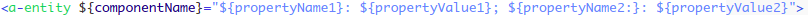
\includegraphics[scale=0.53]{img/entidad1.png}

En un ejemplo lo veremos mejor:

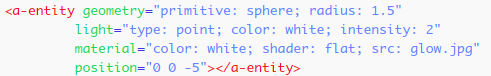
\includegraphics[scale=0.7]{img/entidad.png}\\
\\
Aquí tenemos un objeto primitivo esfera, con un radio de 1.5, el cuál tiene un punto de luz blanco con intensidad 2, sin sombras. La esfera tendrá una textura que se carga mediante la propiedad src de material.
    
    \item  Componentes: Son las propiedades que hacen que una entidad sea diferente a otra.Los componentes donan a la entidad de comportamiento, apariencia y funcionalidad.
    \\Los componentes son módulos de JavaScript que se pueden mezclar, combinar y componer en entidades para crear apariencia, comportamiento y funcionalidad. Podemos registrar un componente en JavaScript y usarlo de forma declarativa desde el DOM.\\ Los componentes son configurables, reutilizables y compartibles. La mayor parte del código en una aplicación A-Frame debería vivir dentro de los componentes.
    
    Podemos utilizar componentes que ya esten creados , o crear nuestros componentes con los parametros y funciones que nos interesen para nuestro programa.
    
    Este es uno de los componentes que he creado en mi programa, cuya funcion es cada vez que le llamamos crea un cartel con los datos que le llegan :
    
    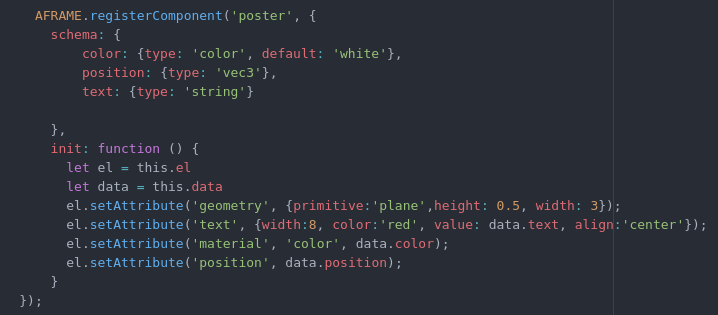
\includegraphics[scale=0.6]{img/componente.png}\\
    
    \item  Sistemas: provienen el entorno donde manejar y desarrollar los componentes. Podemos usar los sistemas para separar la funcionalidad de la información, donde los componentes son los contenedores de la información y el sistema se ocupa de la lógica del uso de estos.

\end{itemize}

A-Frame es compatible con la mayoría de los cascos de realidad virtual como Vive, Rift, Windows Mixed Reality, Daydream, GearVR, Cardboard, Oculus Go e incluso se puede utilizar para la realidad aumentada. Aunque A-Frame admite todo el espectro, A-Frame tiene como objetivo definir experiencias de realidad virtual interactivas totalmente inmersivas que van más allá del contenido básico de 360 °, haciendo un uso completo del seguimiento posicional y los controladores.
\\
\\
\\
A continuación podemos ver un ejemplo simple, el tipico (Hola Mundo) en A-Frame:

  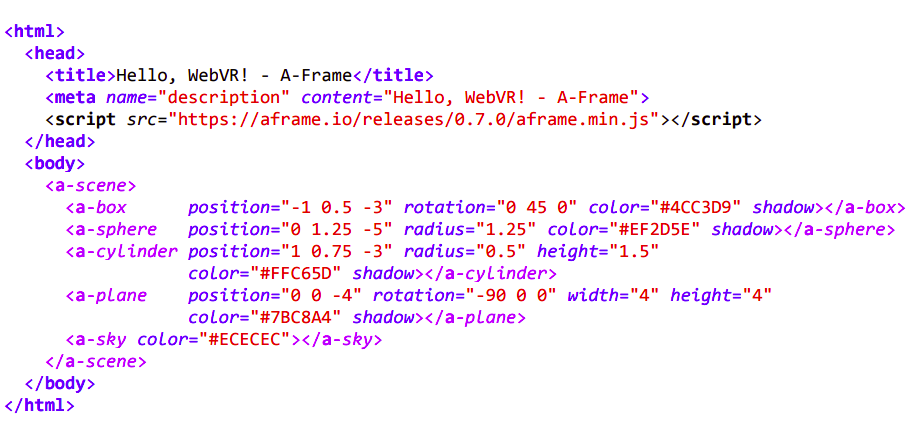
\includegraphics[scale=0.49]{img/code_escena1.png}
 
 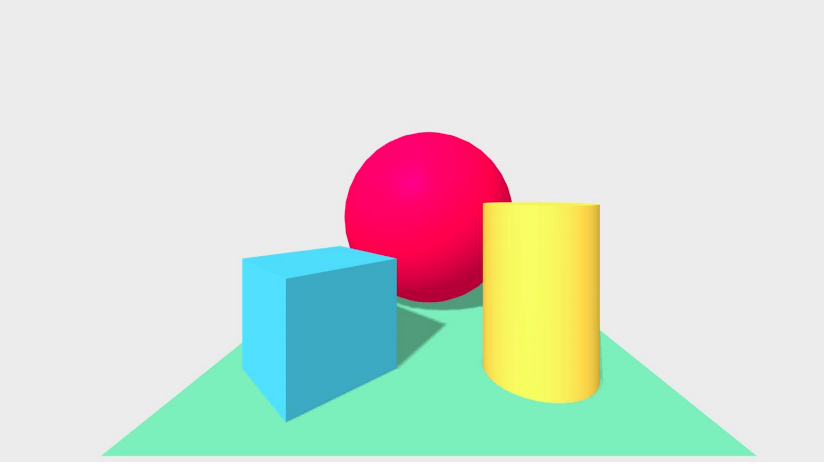
\includegraphics[scale=0.5]{img/escena1.png}


\section{Javascript} 
\label{sec:javascript}

Como hemos visto anteriormente, el lenguaje que más se utiliza en A-frame es Javascript y su DOM.
Ahora veremos en que se fundamenta este lenguaje, y la importancia que tiene en el proyecto.


JavaScript es un lenguaje poderoso, capaz de aportar soluciones eficaces en la mayoría de los ámbitos de la tecnología.
Es especialmente importante porque es el único lenguaje de programación que entienden los navegadores de forma nativa (lenguaje interpretado sin necesidad de compilación), con el que se desarrolla la parte de la funcionalidad frontend en sitios web y aplicaciones web modernas. Por tanto se utiliza como complemento de HTML y CSS para crear páginas webs. Pero también es fundamental en muchos otros tipos de desarrollos.\\
JavaScript es el lenguaje de programación encargado de dotar de mayor interactividad y dinamismo a las páginas web. Cuando JavaScript se ejecuta en el navegador, no necesita de un compilador. El navegador lee directamente el código, sin necesidad de terceros. Por tanto, se le reconoce como uno de los tres lenguajes nativos de la web junto a HTML (contenido y su estructura) y a CSS (diseño del contenido y su estructura).\\

Sus usos más importantes son los siguientes:
\begin{itemize}
    
    \item  Desarrollo de sitios web del lado del cliente (frontend, en el navegador)
    \item  Desarrollo de todo tipo de aplicaciones gracias a la plataforma NodeJS
    \item  Desarrollo de aplicaciones para dispositivos móviles, híbridas o que compilan a nativo
    \item  Desarrollo de aplicaciones de escritorio para sistemas Windows, Linux y Mac, pudiendo escribir un código compatible con todas las plataformas.


    
\end{itemize}
Por tanto, podemos considerar a JavaScript el lenguaje universal, pues es el que más tipos de aplicaciones y usos que puede abarcar en la actualidad. Es por ello que resulta un lenguaje muy recomendable para aprender, ya que nos ofrece capacidades para usarlo en todo tipo de proyectos, siendo que algunos de ellos son parcela exclusiva de JavaScript.

La librería de JavaScript más utilizada en la historia, y que todavía se sigue utilizando es jQuery. Con jQuery podíamos hacer más cosas, escribiendo menos. Con una sintaxis mucho más sencilla, podíamos modificar nuestro sitio web, crear plugins, animar videojuegos y muchas cosas más.
\\

Una de las mayores potencialidades de JavaScript es que puede manipular cualquier elemento de una página web y modificar su contenido, su tamaño, su color, su posición... e incluso hacer aparecer y desaparecer elementos.Para hacer esto posible necesitamos identificar con precisión cada elemento de una página web para poder indicarle a JavaScript sobre qué elemento debe operar.


\section{DOM} 
\label{sec:DOM}
Para permitir que los lenguajes de programación pudieran extraer información o manipular cualquier elemento de una página web era necesario definir de alguna manera qué tipos de elementos conforman una página web, cómo nombrarlos y cómo se relacionan entre sí. Inicialmente esto resultaba bastante problemático, ya que no existía un estándar o especificación oficial sobre cómo debía realizarse esto.

Para evitar los problemas de falta de estandarización, un organismo internacional (el W3C) definió un estándar denominado DOM ó Document Object Model (Modelo de objetos para representar documentos) que define qué elementos se considera que conforman una página web, cómo se nombran, cómo se relacionan entre sí, cómo se puede acceder a ellos, etc...

Las siglas DOM significan Document Object Model, o lo que es lo mismo, la estructura del documento HTML. Una página HTML está formada por múltiples etiquetas HTML, anidadas una dentro de otra, formando un árbol de etiquetas relacionadas entre sí, que se denomina árbol DOM (o simplemente DOM).

En Javascript, cuando nos referimos al DOM nos referimos a esta estructura, que podemos modificar de forma dinámica desde Javascript, añadiendo nuevas etiquetas, modificando o eliminando otras, cambiando sus atributos HTML, añadiendo clases o cambiando el contenido de texto entre otras cosas.


Al estar “amparado” por un lenguaje de programación, todas estas tareas se pueden automatizar, incluso indicando que se realicen cuando el usuario haga acciones determinadas, como por ejemplo: pulsar un botón, mover el ratón, hacer click en una parte del documento, escribir un texto, etc...


\section{Three.js} 
\label{sec:Three}


ThreeJS es una librería JavaScript para el manejo de escenas 3D dentro del canvas del DOM. Por debajo usa WebGL para ofrecer toda su potencia y rendimiento pero con una API mucho más sencilla de usar para el desarrollador.
\newpage

ThreeJS es open source, creada en 2010 y es una de las librerías más populares para crear este tipo de escenas 3D.
Lo bueno de esta librería es que ofrece un montón de utilidades y abstracciones propias de motores 3D: cámaras, objetos, escenas, animaciones, materiales, luces, texturas, etc.

Dado que three.js se basa en JavaScript, es relativamente fácil agregar interactividad entre objetos 3D e interfaces de usuario como el teclado y el mouse. Entonces three.js es perfectamente adecuado para hacer un juego 3D en una plataforma web.

Vamos a ver como poder crear un pequeño programa para ver su utilización.

Primeramente, para cualquier programa o proyecto que empecemos debemos de crear una escena. La escena es como un universo donde podemos agregar objetos, cámaras y luces, etc.
\begin{center}
var scene = new THREE.Scene();
\end{center}
A continuación tenemos que configurar la cámara, hay cámaras en perspectiva y ortográficas. Durante la mayor parte del tiempo, mantendremos la perspectiva, que es un tipo de cámara normal en el que verá objetos más cercanos, más grandes y más pequeños, cuando estén lejos.

Para la cámara de ortografía, verá una vista isométrica de un ángulo específico sin perspectiva.
Entonces el primer parámetro de la cámara es el campo de visión, básicamente es el ancho del ángulo de percepción. Configurémoslo en 75, la siguiente es la relación de aspecto, vamos a usar el ancho actual dividido por la altura.
\begin{center}

var camera = new THREE.PerspectiveCamera(75,window.innerWidth/window.innerHeight);
\end{center}

Después, vamos a configurar el renderizador. Usaremos el renderizador WebGL.Puede personalizar la opción de representación aquí, como anti-aliasing. 
\begin{center}
var renderer = new THREE.WebGLRenderer({antialias: true});

\end{center}
Una vez creada la escena y configurada la cámara, podemos empezar a crear los objetos que queramos introducir en ella. 

A continuación vamos a crear un cubo.
Lo primero es crear una geometría, pensar en ella como un esqueleto para nuestro objeto. Hay muchos tipos de geometría disponibles, pero como vamos a crear un cubo, usaremos BoxGeometry con el mismo tamaño en todas las dimensiones.

\begin{center}
var geometry = new THREE.BoxGeometry(1,1,1);
\end{center}

Ahora vamos a necesitar una textura para caracterizar nuestra geometría. Así que necesitamos material que defina las características de la piel, como la opacidad, el reflejo o la textura. Usemos MeshBasicMaterial (color sólido sin reflexión y cálculo de iluminación) con color rojo por ahora.
\begin{center}
var material = new THREE.MeshBasicMaterial({color: 0xff0000});
\end{center}
Ahora podemos crear nuestro cubo creando un objeto de malla usando nuestra geometría y material y agregando el cubo a la escena.
\begin{center}
var cube = new THREE.Mesh(geometry,material);
scene.add(cube);

\end{center}
Pero como acabamos de agregar todo a la escena sin especificar la posición, ahora nuestro cubo está en el mismo lugar que la cámara y no se procesará. Lo colocamos en una posición de la escena que se vea y lo rotamos para que se vea como nos interese:

\begin{center}
cube.position.z = -5;
cube.rotation.x = 10;
cube.rotation.y = 5;
\end{center}

Ahora llamamos a un método de renderizado en el objeto renderizador y le pasamos la escena y la cámara.
\begin{center}
renderer.render(scene,camera);
\end{center}

Con esto, ya tendríamos el cubo creado e incluido en la escena y ya estaría renderizado. Podemos incluir también una animación como la rotación a nuestro cubo para que aparezca moviéndose y ya tendríamos nuestro primer pequeño programa.

\begin{figure}
\centering
 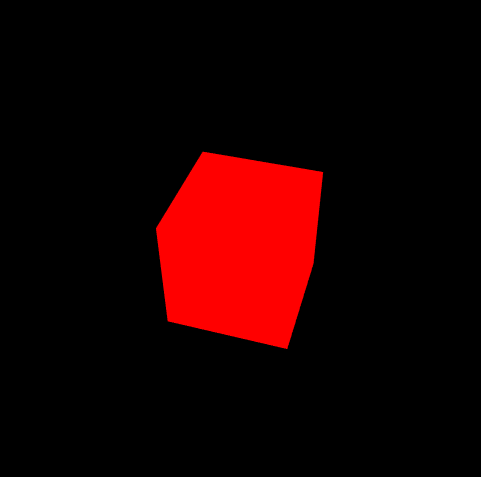
\includegraphics[scale=0.5]{img/threejs-renderizadocubo.png}
\end{figure}

\begin{figure}
\centering
 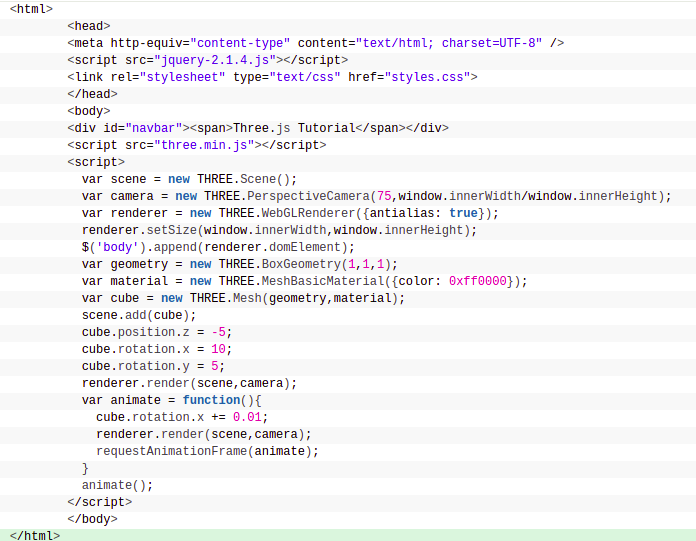
\includegraphics[scale=0.6]{img/codigoThree.png}
\end{figure}


\newpage
\section{WebGL} 
\label{sec:WebGL}


WebGL es una especificación estándar que está siendo desarrollada actualmente para desplegar gráficos en 3D en navegadores web. El WebGL permite activar gráficos en 3D acelerados por hardware en páginas web, sin la necesidad de plug-ins en cualquier plataforma.

A grandes rasgos, WebGL es un mecanismo que tienen los navegadores para usar toda la potencia de la tarjeta gráfica de los usuarios que visitan las páginas web para poder pintar escenas en 3D.
Antiguamente, antes de que existiera WebGL se usaba la propia API del canvas del DOM y Flash lo que hacía que las escenas 3D fueran muy simples.

Hoy en día, con WebGL puedes crear escenas 3D complejas, ya que todo se va a renderizar en la tarjeta gráfica del usuario que entre en la web (queda en manos del programador ajustar la calidad de los gráficos dependiendo de la potencia de la tarjeta gráfica del usuario).

WebGL creció desde los experimentos del canvas 3D comenzados por Mozilla. Mozilla primero demostró un prototipo de Canvas 3D en 2006. A finales de 2007, tanto Mozilla como Opera habían hecho sus propias implementaciones separadas. A principio de 2009 Mozilla y Khronos comenzaron el WebGL Working Group (Grupo de Trabajo del WebGL). El Grupo de Trabajo del WebGL incluye Apple, Google, Mozilla, y Opera, y WebGL.

Para usar WebGL no necesitas ningún framework, lo puedes hacer con Javascript sin instalar nada, pero programar en WebGL es tan complejo que lo mejor es usar alguna librería tipo ThreeJS o PixiJS para facilitar la tarea de programación.

\newpage
\section{WebXR} 
\label{sec:WebXR}
WebXR  es un grupo de estándares que se utilizan juntos para admitir la representación de escenas 3D en hardware diseñado para presentar mundos virtuales (realidad virtual o  VR) o para agregar imágenes gráficas al mundo real ( realidad aumentada o  AR ).  Las  API de Dispositivos WebXR implementa el núcleo del conjunto de características WebXR, la gestión de la selección de los dispositivos de salida, hacen que la escena 3D en el dispositivo elegido a la tasa de trama adecuado y administrar vectores de movimiento creados utilizando controladores de entrada.

Los dispositivos compatibles con WebXR incluyen auriculares 3D totalmente inmersivos con seguimiento de movimiento y orientación, anteojos que superponen gráficos sobre la escena del mundo real que pasa a través de los marcos y teléfonos móviles de mano que aumentan la realidad al capturar el mundo con una cámara y aumentar esa escena con una computadora. 

Para lograr estas cosas, la API del dispositivo WebXR proporciona las siguientes capacidades clave:

\begin{itemize}
    \item Encuentra dispositivos de salida de realidad virtual o realidad aumentada compatibles.
    \item Renderice una escena 3D en el dispositivo a una velocidad de fotogramas adecuada.
    \item (Opcionalmente) refleje la salida en una pantalla 2D. 
    \item Crear vectores que representen los movimientos de los controles de entrada.

\end{itemize}
En el nivel más básico, una escena se presenta en 3D calculando la perspectiva a aplicar a la escena con el fin de renderizarla desde el punto de vista de cada uno de los ojos del usuario calculando la posición de cada ojo y renderizando la escena desde esa posición, mirando en la dirección en la que se encuentra el usuario. Cada una de estas dos imágenes se renderiza en un solo framebuffer, con la imagen renderizada del ojo izquierdo a la izquierda y el punto de vista del ojo derecho renderizado en la mitad derecha del buffer. Una vez que se han representado las perspectivas de ambos ojos sobre la escena, el framebuffer resultante se envía al dispositivo WebXR para que se lo presente al usuario a través de sus auriculares u otro dispositivo de visualización apropiado.

\section{HTML5} 
\label{sec:HTML5}

HTML5 es la quinta versión del lenguaje de programación HTML (HyperText Markup Language) que mejora y aprovecha todo el potencial de la Word Wide Web (WWW).
El término representa dos conceptos diferentes:
\begin{itemize}
    \item Se trata de una nueva versión de HTML, con nuevos elementos, atributos y comportamientos.
    \item Contiene un conjunto más amplio de tecnologías que permite a los sitios Web y a las aplicaciones ser más diversas y de gran alcance. A este conjunto se le llama HTML5 y amigos, a menudo reducido a HTML5 .
\end{itemize}
Diseñado para ser utilizable por todos los desarrolladores de Open Web, esta página referencía numerosos recursos sobre las tecnologías de HTML5, clasificados en varios grupos según su función.

Para entender de forma sencilla en qué consiste HTML5 debemos explicar que ofrece funcionalidades que mejoran la experiencia de navegación, es decir, los diferentes navegadores (Chrome, Explorer, Safari o Firefox) entienden rápidamente como está estructurada una web y cuáles son los elementos que la componen, aunque esto ya lo incorporaba la versión anterior, ahora se pueden incluir nuevos elementos, reduciendo el uso de plugins y mejorando la velocidad de carga.

Se trata de una nueva versión de HTML, con nuevos elementos, atributos y comportamientos. Contiene un conjunto más amplio de tecnologías que permite a los sitios Web y a las aplicaciones ser más diversas y de gran alcance.

Algunas de las nuevas características de HTML5 serían:
\begin{itemize}


    \item Semántica: Permite describir con mayor precisión cuál es su contenido.
    
    \item Conectividad: Permite comunicarse con el servidor de formas nuevas e innovadoras.
    
    \item Sin conexión y almacenamiento: Permite a las páginas web almacenar datos localmente en el lado del cliente y operar sin conexión de manera más eficiente.
    
    \item Multimedia: Nos otorga un excelente soporte para utilizar contenido multimedia como lo son audio y video nativamente.
    
    \item Gráficos y efectos 2D/3D: Proporciona una amplia gama de nuevas características que se ocupan de los gráficos en la web como lo son canvas 2D, WebGL, SVG, etc.
    
    \item Rendimiento e Integración: Proporciona una mayor optimización de la velocidad y un mejor uso del hardware.
    
    \item Acceso al dispositivo: Proporciona APIs para el uso de varios componentes internos de entrada y salida de nuestro dispositivo.
    
    \item CSS3: Nos ofrece una nueva gran variedad de opciones para hacer diseños más sofisticados.

    \item Nuevas etiquetas semánticas para estructurar los documentos HTML, destinadas a remplazar la necesidad de tener una etiqueta $<$div$>$que identifique cada bloque de la página.
    
    \item Los nuevos elementos multimedia como$<$audio$>$ y $<$video$>$.
    
    \item La integración de gráficos vectoriales escalables (SVG) en sustitución de los genéricos $<$object$>$, y un nuevo elemento $<$canvas$>$; que nos permite dibujar en él.

    \item El cambio, redefinición o estandarización de algunos elementos, como $<$a$>$, $<$cite$>$ o $<$menu$>$.
    
    \item MathML para fórmulas matemáticas.
    
    \item Almacenamiento local en el lado del cliente.
    \newline
\end{itemize}

El funcionamiento HTML5 consiste en un proceso que solicita una página HTML a través del navegador.

Desde el navegador se realiza una petición a un servidor, lo que se hace a través de una dirección del tipo http://..../index.html. Después el servidor recupera de su disco duro esa página, la devuelve al navegador y la página se muestra.

\newpage
\section{Github} 
\label{sec:Github_info}

GitHub es un servicio basado en la nube que aloja un sistema de control de versiones (VCS) llamado Git. Este permite a los desarrolladores colaborar y realizar cambios en proyectos compartidos, a la vez que mantienen un seguimiento detallado de su progreso. Fue comprada por Microsoft en junio del 2018. 

La plataforma está creada para que los desarrolladores suban el código de sus aplicaciones y herramientas, y que como usuario no solo puedas descargarte la aplicación, sino también entrar a su perfil para leer sobre ella o colaborar con su desarrollo.

Como su nombre indica, la web utiliza el sistema de control de versiones Git diseñado por Linus Torvalds. Un sistema de gestión de versiones es ese con el que los desarrolladores pueden administrar su proyecto, ordenando el código de cada una de las nuevas versiones que sacan de sus aplicaciones para evitar confusiones. Así, al tener copias de cada una de las versiones de su aplicación, no se perderán los estados anteriores cuando se va a actualizar.

Esto significa que cualquier desarrollador del equipo que tenga acceso puede gestionar el código fuente y su historial de cambios utilizando las herramientas de línea de comandos de Git.

A diferencia de los sistemas de control de versiones centralizados, Git ofrece ramas de características. Con lo que cada ingeniero de software en el equipo puede dividir una rama de características que proporcionará un repositorio local aislado para hacer cambios en el código.

Las ramas de características no afectan a la rama maestra, que es donde se encuentra el código original del proyecto. Una vez que se hayan realizado los cambios y el código actualizado esté listo, la rama de características puede fusionarse de nuevo con la rama maestra, que es la forma en que se harán efectivos los cambios en el proyecto.

Además, la interfaz de usuario de GitHub es más fácil de usar que la de Git, lo que la hace accesible para personas con pocos o ningún conocimiento técnico. Esto significa que se puede incluir a más miembros del equipo en el progreso y la gestión de un proyecto, haciendo que el proceso de desarrollo sea más fluido.
Las principales características de la plataforma es que ofrece las mejores características de este tipo de servicios sin perder la simplicidad, y es una de las más utilizadas del mundo por los desarrolladores. Es multiplataforma, y tiene multitud de interfaces de usuario.


\newpage
\section{Atom} 
\label{sec:Atom}

Atom es un editor de código de fuente abierta para macOS, Linux, y Windows con soporte para plug-ins escrito en Node.js, Incrustando Git Control, desarrollado por GitHub. Es una aplicación de escritorio construida utilizando tecnologías web.

Está basado en Electrón (Anteriormente conocido como Atom Shell), Un framework que permite aplicaciones de escritorio multiplataforma usando Chromium y Node.js. También puede ser utilizado como un entorno de desarrollo integrado (IDE).

Sus características principales son:
\begin{itemize}
    \item Sirve para trabajar en cualquier sistema operativo (Windows, OS X o Linux).
    \item Puedes instalarle paquetes o crear los tuyos propios.
    \item Autocompletado inteligente que permite escribir código más rápido.
    \item Buscar y reemplazar texto de una forma sencilla.
\end{itemize}

Este editor de código nos facilita la manera de programar ayudándonos a autocompletar algunos campos, y también nos facilita sobre todo a incluir nuestro código en nuestro repositorio de Github e ir actualizandolo de manera muy sencilla.

\begin{figure}[h]
\centering
 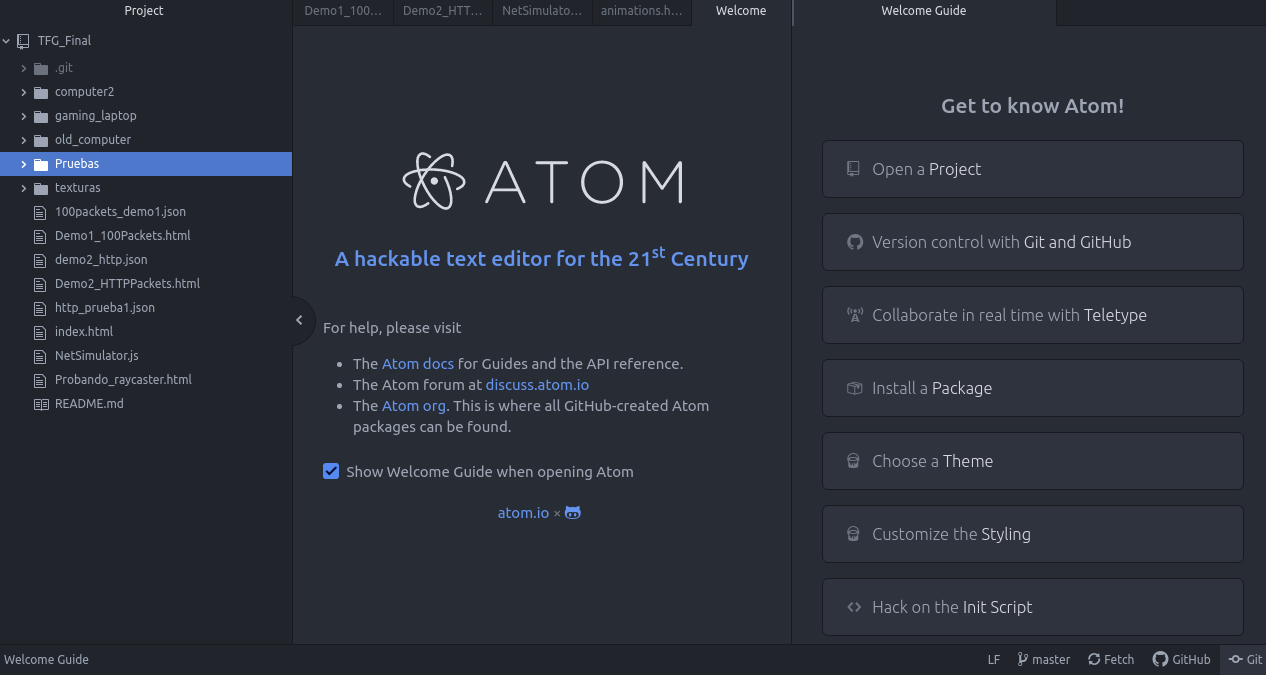
\includegraphics[scale=0.35]{img/github.png}
\end{figure}


\newpage
\section{LaTeX} 
\label{sec:LaTeX}


LaTeX, es un sistema que ayuda al usuario a preparar un documento. Con él puedes preparar cualquier tipo de documento para presentarlo tanto en papel como en pantalla tales como manuscritos, cartas, artículos de revistas y tesis.

La historia de LaTeX empieza con TeX, un sistema de tipografía creado por Donald E. Knuth y publicado por primera vez en 1978. Su propósito era ayudar a matemáticos, físicos e informáticos en la composición de sus textos, que habitualmente incluían nomenclatura compleja.

LaTeX es una mejora o evolución de TeX, creado por Leslie Lamport en 1984, y que emplea macros de TeX para emplear composición tipográfica de una manera más simple que con el TeX original. 
Además de para emplear notación matemática o científica de manera más cómoda que con un editor de texto genérico, también permite aplicar elementos de formato como notas al pie, índices o capítulos.

La calidad de imprenta de LaTeX pueden ser usados en áreas como química, física, computación, biología, leyes, literatura, música y en cualquier otro tema el cual usen simbologías.
Otra característica es que te permite separar el contenido y el formato del documento. Así tener la oportunidad de concentrarte en generar y escribir ideas en una parte y plasmar esas ideas en otra.

Otra ventaja es que los textos creados con LaTeX son compatibles con cualquier sistema operativo o plataforma, y que pueden exportarse a formatos populares como PDF, HTML, RTF o Postscript, entre otros.


\newpage
\section{Realidad Virtual} 
\label{sec:VR}

La realidad virtual (VR) consiste en la inmersión sensorial en un nuevo mundo, basado en entornos reales o no, que ha sido generado de forma artificial, y que podemos percibir gracias a unas gafas de realidad virtual y sus accesorios (cascos de audio, guantes, etc…).

El objetivo de esta tecnología es crear un mundo ficticio del que puedes formar parte e incluso ser el protagonista: viendo un coche en un concesionario virtual, siendo protagonista de un videojuego o bien practicando como hacer una operación a corazón abierto.

 En estas experiencias de realidad virtual puedes interactuar y explorar. Es el usuario quien controla la escena y puede interactuar con los objetos de la misma.

A diferencia de la realidad aumentada, que mejora la realidad sensorialmente, pero que es una realidad mixta entre el mundo real y el virtual, la realidad virtual debe ser inmersiva, permitir la interacción y tener una historia que respalde esa realidad.

 La medicina, la cultura, la educación y la arquitectura son algunos de los ámbitos que ya han sucumbido a las ventajas que ofrece esta tecnología. Desde visitas guiadas a museos hasta la disección de un músculo, la RV nos permite cruzar unos límites que de otra forma no serían imaginables.
\\
\begin{figure}[h]
\centering
 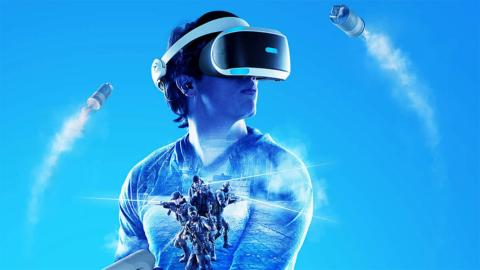
\includegraphics[scale=1]{img/VR.jpg}
\end{figure}
%%%%%%%%%%%%%%%%%%%%%%%%%%%%%%%%%%%%%%%%%%%%%%%%%%%%%%%%%%%%%%%%%%%%%%%%%%%%%%%%
%%%%%%%%%%%%%%%%%%%%%%%%%%%%%%%%%%%%%%%%%%%%%%%%%%%%%%%%%%%%%%%%%%%%%%%%%%%%%%%%
% DISEÑO E IMPLEMENTACIÓN %
%%%%%%%%%%%%%%%%%%%%%%%%%%%%%%%%%%%%%%%%%%%%%%%%%%%%%%%%%%%%%%%%%%%%%%%%%%%%%%%%

\cleardoublepage
\chapter{Diseño e implementación}

En este capítulo hablaré del diseño e implementación del proyecto. Trataré el tema de la metodología que he utilizado e iré viendo todas las etapas hasta llegar al resultado final.

\section{Metodología ágil SCRUM} 
\label{sec:met_agil}
En este proyecto he utilizado una versión muy simplificada de SCRUM para desarrollar el trabajo a través de sprint y facilitar con ello la construcción del programa.

La metodología SCRUM es un marco de trabajo o framework que se utiliza dentro de equipos que manejan proyectos complejos. Es decir, se trata de una metodología de trabajo ágil que tiene como finalidad la entrega de valor en períodos cortos de tiempo y para ello se basa en tres pilares: la transparencia, inspección y adaptación. Esto permite al cliente, junto con su equipo comercial, insertar el producto en el mercado pronto, rápido y empezar a obtener ventas.

Con la metodología SCRUM, el equipo tiene como foco entregar valor y ofrecer resultados de calidad que permitan cumplir los objetivos de negocio del cliente.

Para ello, los equipos de SCRUM son autoorganizados y multifuncionales. Es decir, cada uno es responsable de unas tareas determinadas y de terminarlas en los tiempos acordados. Esto garantiza la entrega de valor del equipo completo, sin necesidad de ayuda o la supervisión minuciosa de otros miembros de la organización.

En SCRUM existen 3 roles muy importantes: Product Owner, SCRUM Master y Equipo de desarrollo.
\begin{itemize}
\newpage
    \item Product owner:
    Es el responsable de maximizar el valor del trabajo del equipo de desarrollo. La maximización del valor del trabajo viene de la mano de una buena gestión del Product Backlog.
    El Product owner es el único perfil que habla constantemente con el cliente, lo que le obliga a tener muchos conocimientos sobre negocio.
    Para finalizar, un equipo SCRUM debe tener solo un Product Owner y este puede ser parte del equipo de desarrollo.
    
    \item SCRUM Master:
    Es el responsable de que las técnicas SCRUM sean comprendidas y aplicadas en la organización. Es el manager de SCRUM, un líder que se encarga de eliminar impedimentos o inconvenientes que tenga el equipo dentro de un, aplicando las mejores técnicas para fortalecer el equipo de marketing digital.
    Dentro de la organización, el SCRUM Master tiene la labor de ayudar en la adopción de esta metodología en todos los equipos.
    
    \item Equipo de desarrollo:
    Son los encargados de realizar las tareas priorizadas por el Product Owner. Es un equipo multifuncional y autoorganizado. Son los únicos que estiman las tareas del product backlog, sin dejarse influenciar por nadie.
    Los equipos de desarrollo no tienen sub-equipos o especialistas. La finalidad de esto es transmitir la responsabilidad compartida si no se llegan a realizar todas las tareas de un sprint.
    
\end{itemize}

En este proyecto,voy a actuar como desarrollador, y el rol de SCRUM Master y Product owner será los que tome mi tutor Jesus María González Barahona.

El núcleo central de la metodología de trabajo ‘SCRUM’ es el ‘sprint’. Se trata de un miniproyecto, cuyo objetivo es conseguir un incremento de valor en el producto que estamos construyendo. Todo ‘sprint’ cuenta con una definición y una planificación que ayudará a lograr las metas marcadas.

El primer paso para alcanzar este objetivo -o hito del proyecto- es la reunión de planificación, una sesión en la que debe participar todo el equipo ‘SCRUM’ y que supone el pistoletazo de salida del ‘sprint’. Esta reunión se divide en dos partes que tratan de dar respuesta a dos preguntas fundamentales: ¿Qué se va a entregar?, y ¿cómo se va a realizar el trabajo?

Cuando el ‘sprint’ ha comenzado, cada uno de los miembros del equipo ejerce su rol, asegurándose de que se cumplan siempre las siguientes condiciones:
\begin{itemize}
\newpage
    \item No se realizan cambios que pongan en peligro el objetivo.
    \item Los estándares de calidad no disminuyen.
    \item El ‘Product owner’ y el equipo de desarrollo trabajan conjuntamente ajustando el detalle de las funcionalidades planificadas para el ‘sprint’.
    \item Además de construir el producto, todo equipo trabaja conjuntamente en la redefinición del proyecto. El ‘Product owner’ y los miembros del equipo aclaran y negocian entre ellos a medida que se aprende más.

\end{itemize}

Al final de cada ‘sprint’ se lleva a cabo una labor de inspección y revisión del trabajo realizado, en la que el ‘Product owner’ (o incluso el propio cliente) da ‘feedback’ al equipo. En esta sesión, el propietario del producto decide si se acepta o no como válida la funcionalidad o entregable desarrollado. La reunión debe cumplir una serie de condiciones:

\begin{itemize}
    \item Los asistentes somos, mi tutor del proyecto y yo.
    \item Se identifica lo que se ha hecho durante la semana anterior y los avances que ha habido.
    \item Se detectan los problemas y se analiza cómo se resolvieron.
    \item Vemos hacia donde podemos orientar el proyecto, y cuáles son los siguientes pasos a seguir.
\end{itemize}
Todas las metodologías ágiles buscan mejorar de manera continua la forma en la que el equipo se relaciona durante el proceso de desarrollo. 


\section{ETAPAS} 
\label{sec:estapas}

\subsection{Etapa 0: Aprendizaje}

Esta etapa es fundamental y una de las más importantes en el desarrollo del proyecto.
En esta etapa tuve que aprender desde 0 todo sobre la tecnología A-frame, ya que no tenía ninguna noción de esta tecnología, y gracias a la documentación
\footnote{\url{https://aframe.io/docs/1.1.0/introduction/}}, ejemplos
\footnote{\url{https://aframe.io/}} y tutoriales conseguí aprender y poder construir escenas en realidad virtual.

Para poner todo esto en práctica e inicializarme en el mundo de A-Frame, construí una escena con varias animaciones, texturas, luces y una componente que tiene varias propiedades, que es la que se muestra a continuación:

\begin{figure}[h]
\centering
    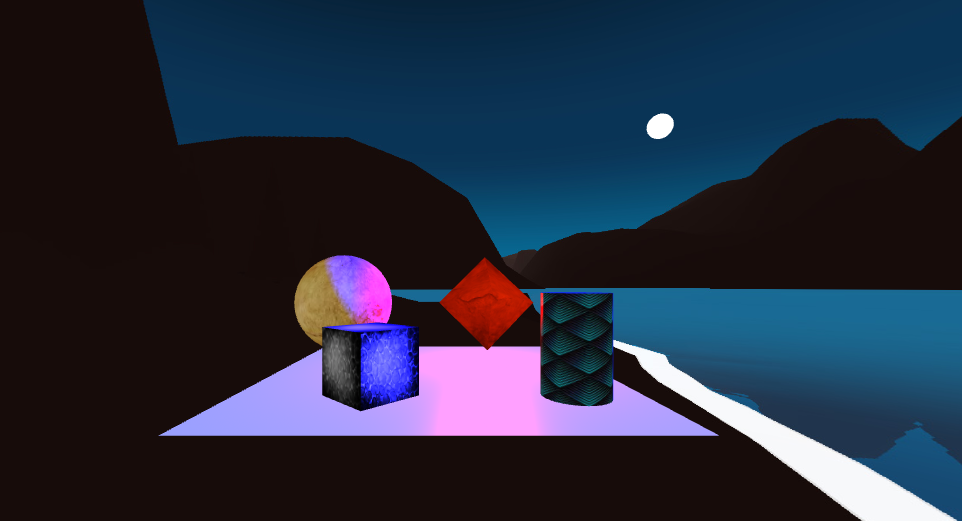
\includegraphics[scale=0.45]{img/escena0.png}
\end{figure}
Después de todas estas pruebas llegamos a la creación de nuestra primera escena\footnote{\url{https://alejandroeslo.github.io/TFG/Pruebas/Pasos_seguidos/P1.html}} del proyecto, que está compuesta por 2 ordenadores que se intercambian los 7 paquetes que indicábamos anteriormente(3 paquetes de señalización(SYN), 2 paquetes de datos y otros 2 paquetes de Fin de conexión) al pulsar el botón azul.


En esta escena podemos ver varios elementos que la componen, y algunos de ellos tienen asociada una animación.
Si visitáis la escena
\footnote{\url{https://alejandroeslo.github.io/TFG/Pruebas/Prueba_inicial/Escena_prueba.html}}, podréis ver las siguientes animaciones:

\begin{itemize}

    \item Una esfera blanca que se comportara como punto de luz y se irá moviendo de un lado a otro.
    
    \item Un octaedro, que está girando constantemente, y al pinchar sobre él, se irá alejando y acercando.
    
    \item La esfera colocada en el plano, al pinchar sobre ella, empezará a rotar y se pondrá de color verde.
    
\end{itemize}

\newpage
\subsection{Etapa 1: Comienzo del proyecto}

Después de haber estado practicando con la escena inicial tras haberme leído y estudiado la documentación de A-Frame y las otras tecnologías necesarias para su elaboración, pasaremos a comenzar a crear nuestro primer programa relacionado con el proyecto.
Este programa será una aplicación sencilla [Cliente – Servidor], y avanzaremos en dos direcciones:


\begin{flushleft}
A-FRAME:
\\
Comenzaremos construyendo una escena en la que tengamos dos cajas iniciales, una será el cliente y otra será el servidor.

Incluiremos 7 paquetes que serán enviados desde el cliente(emisor) hasta el servidor(receptor), estos paquetes los empezaremos introduciendo en una lista en la que distinguiremos 3 paquetes de señalización(SYN), 2 paquetes de datos y otros 2 paquetes de Fin de conexión.

Estos paquetes se enviarán mediante diferentes acciones que definiremos como por ejemplo pulsar una tecla, y haremos que los paquetes se envíen de manera automática o paso a paso(break point).
\end{flushleft}

Resumen:
\begin{itemize}
    \item 2 Cajas (cliente y servidor).
    \item 7 paquetes diferentes que vayan de una caja a otra.
    \item Funcionalidad para movimiento de los paquetes.
\end{itemize}

\begin{flushleft}
WIRESHARK:

Sacar una traza de TCP en formato JSON para poder luego analizarla y ver que campos contiene y poder extraer estos datos mediante Javascript.
\end{flushleft}


Para empezar con ello, primeramente tuve que realizar unas demos para ver como controlar las entidades y gestionar llamadas a los eventos para ver como podía manejar correctamente el movimiento de los paquetes de un ordenador a otro al darle a un botón.

\newpage
Primero comencé por crearme una escena\footnote{\url{https://alejandroeslo.github.io/TFG/Pruebas/Pruebas_eventos/e2.html}} básica donde únicamente tenía un cubo y al pinchar sobre el cubo apareciese una esfera a su lado:

\begin{figure}[h]
\centering
    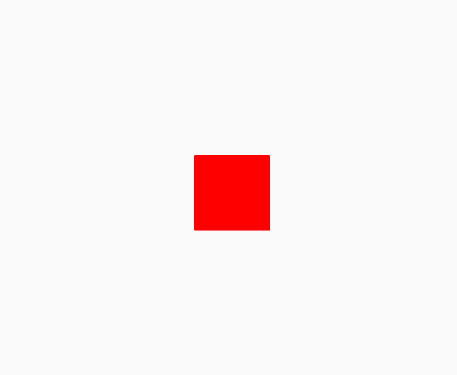
\includegraphics[scale=0.35]{img/escena1_1a.png}
    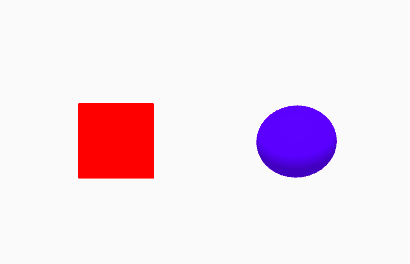
\includegraphics[scale=0.45]{img/escena1_1b.png}
\end{figure}

Con ello comenzamos a ver como se controlan los eventos, y en este ejemplo podemos apreciar el evento creado con la función “ created\_sphere” que nos creara esa esfera azul al pinchar en el cubo.

\begin{figure}[h]
\centering
 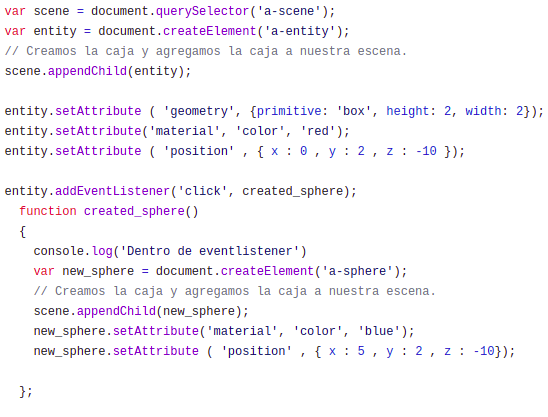
\includegraphics[scale=0.75]{img/code1-1.png}
\end{figure}

\newpage
A continuación pasamos a crear 2 cajas, y al hacer click en una, se cree un evento en la otra. Por lo tanto, ahora en esta nueva escena\footnote{\url{https://alejandroeslo.github.io/TFG/Pruebas/Pruebas_eventos/e3.html}}, al hacer click en la caja roja, la caja verde se convertirá en una esfera amarilla:

\begin{figure}[h]
\centering
    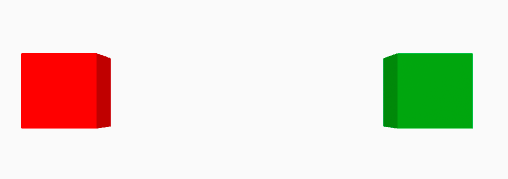
\includegraphics[scale=0.5]{img/escena1_2a.png}
    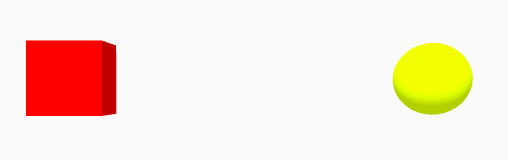
\includegraphics[scale=0.5]{img/escena1_2b.png}
\end{figure}

Ahora podemos ver el evento creado con la función “ change\_box2” que al hacer click en el cubo verde, que es la entidad 2(entity2), se cambiara por una esfera amarilla.

\begin{figure}[h]
\centering
 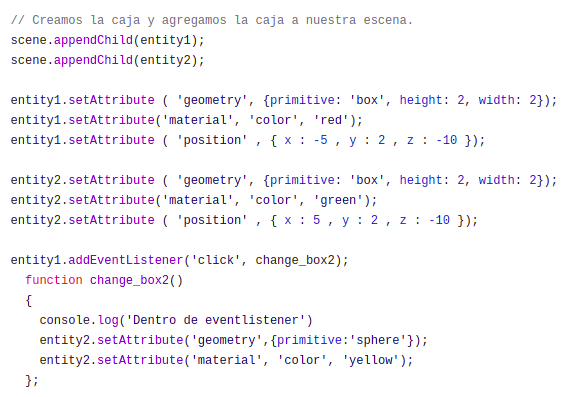
\includegraphics[scale=0.75]{img/escena1-2.png}
\end{figure}

\newpage
Y en la escena\footnote{\url{https://alejandroeslo.github.io/TFG/Pruebas/Pruebas_eventos/e4.html}} final para controlar los eventos pondremos crearemos un componente para usarlo como manejador sobre la escena anterior, que lo que nos permitira sera que al hacer click en la esfera amarilla, esta comenzara una animacion en loop que creara un efecto de que la esfera se aleja y se acerca :

\begin{figure}[h]
\centering
    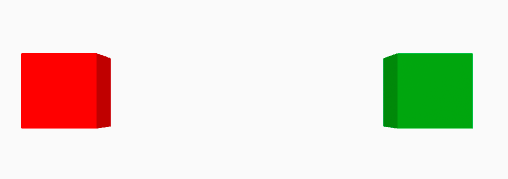
\includegraphics[scale=0.5]{img/escena1_2a.png}
    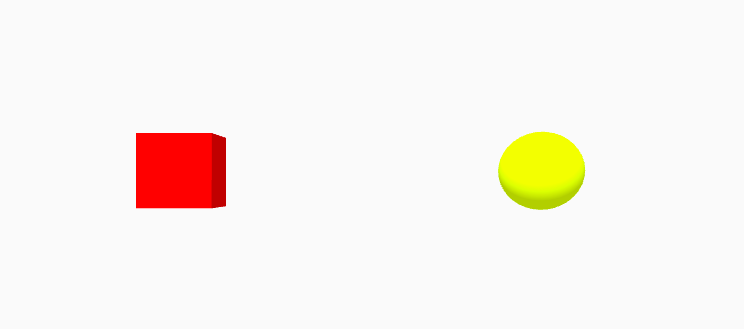
\includegraphics[scale=0.3]{img/escena1_3a.png}
    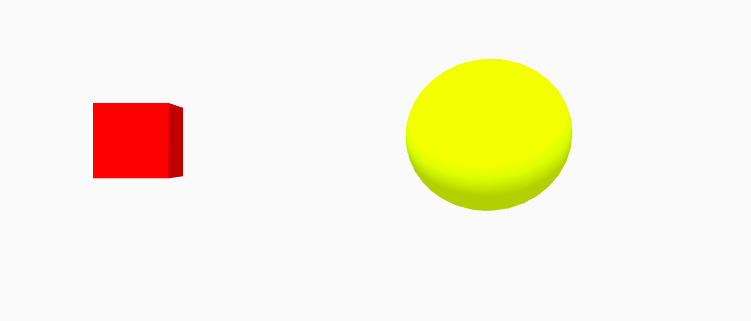
\includegraphics[scale=0.3]{img/escena1_3b.png}
\end{figure}

Ahora podemos ver el evento creado con la función “ change\_box2” ahora incluimos el manejador, que es un componente que hemos creado anteriormente para darle la animación a la esfera amarilla.

\begin{figure}[h]
\centering
 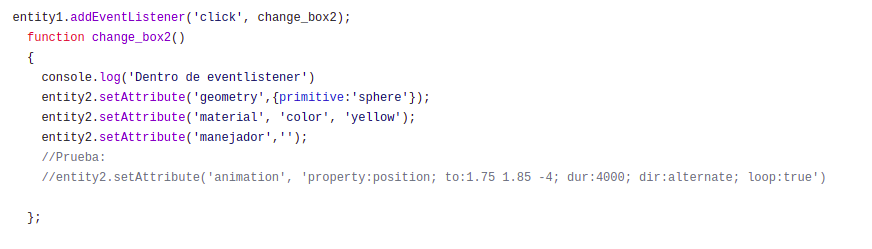
\includegraphics[scale=0.55]{img/code_1-3a.png}
  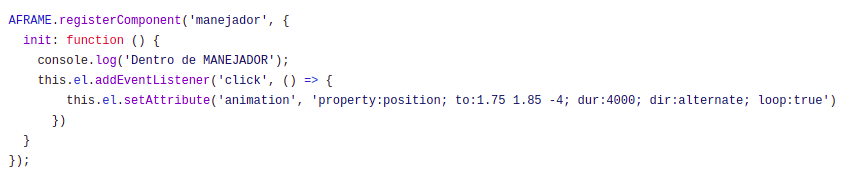
\includegraphics[scale=0.55]{img/code_1-3b.png}
\end{figure}

\newpage
Después de todas estas pruebas llegamos a la creación de nuestra primera escena\footnote{\url{https://alejandroeslo.github.io/TFG/Pruebas/Pasos_seguidos/P1.html}} del proyecto, que está compuesta por 2 ordenadores que se intercambian los 7 paquetes que indicábamos anteriormente(3 paquetes de señalización(SYN), 2 paquetes de datos y otros 2 paquetes de Fin de conexión) al pulsar el botón azul.
Los paquetes empezarán con un color, y una vez que lleguen al destino se volverán verdes.

\begin{figure}[h]
\centering
    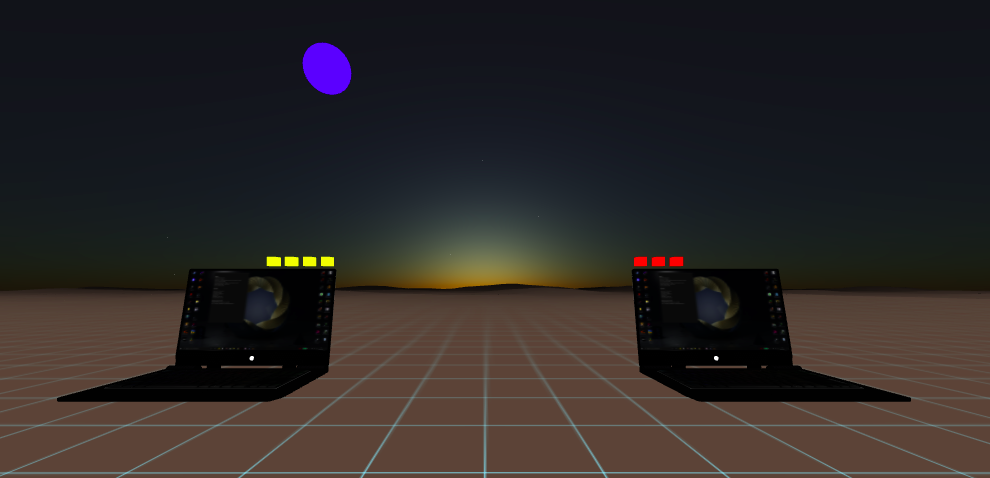
\includegraphics[scale=0.33]{img/escenafinal_1.png}
\end{figure}

\begin{figure}[h]
\centering
    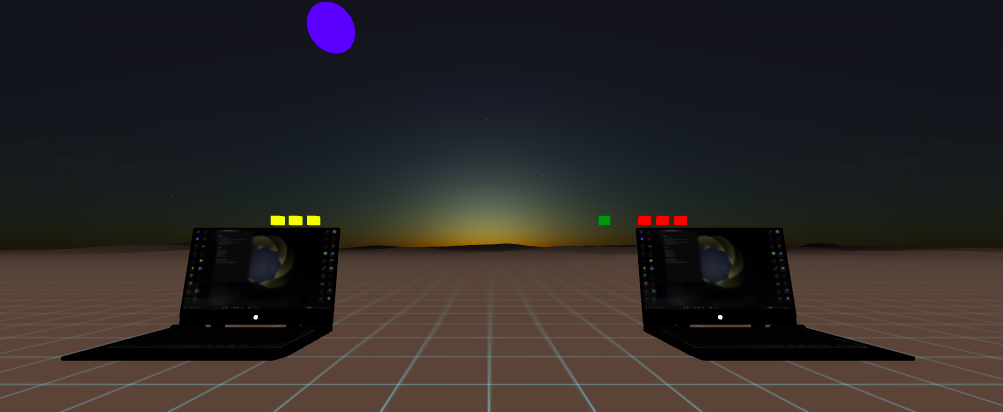
\includegraphics[scale=0.33]{img/escenafinal_2.png}
\end{figure}

\begin{figure}[h]
\centering
    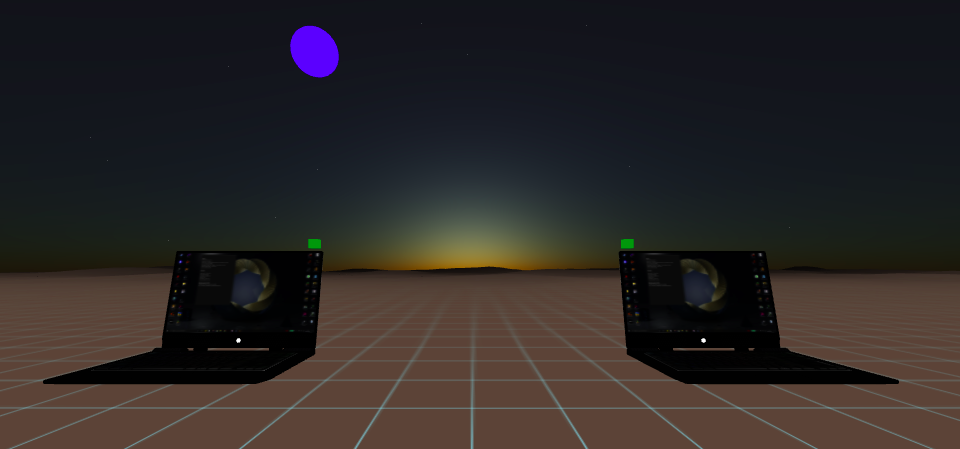
\includegraphics[scale=0.35]{img/escenafinal_3.png}
\end{figure}

\subsection{Etapa 2: Primer prototipo}

Después de haber creado nuestra primera escena con animaciones de los paquetes entre cliente y servidor, ahora vamos a aumentar el número de nodos(ordenadores) y conectarlos entre sí mediante tubos transparentes.Avanzaremos en 2 direcciones diferentes :
\begin{flushleft}
ANIMACIÓN:
\\
Crearemos varios ordenadores mas distribuidos en la escena e interconectados todos a través 	de unos tubos transparentes por los cuales se enviaran y recibirán los paquetes.
\end{flushleft}

\begin{flushleft}
WIRESHARK:

Trataremos de leer las capturas exportadas en JSON desde JavaScript. Para ello lo que 	haremos sera recibir el fichero JSON de la red mediante http y pedir este fichero mediante 	GET para convertirlo después en un objeto y poderlo mostrar por la linea de comandos del 	navegador.

Crearemos un bucle para leer(por ejemplo: las direcciones Ethernet de todos los paquetes de la captura), y después mostrarlos a través de la linea de comandos del navegador

\end{flushleft}

En esta etapa nos centraremos en crear una escena\footnote{\url{https://alejandroeslo.github.io/TFG/Pruebas/Pasos_seguidos/P2.html}} más grande, con mayor número de ordenadores interconectados entre sí a través de tuberías transparentes por las cuales se enviaran los paquetes después de pulsar el botón que iniciara la animación.

Comenzaremos con la creación y colocación de los nodos(ordenadores) con unas posiciones fijas que he calculado para que quede visualmente bien y se puedan ver todos los nodos intercambiar los paquetes. Aqui podemos ver un par de nodos como ejemplo:

\begin{figure}[h]
\centering
    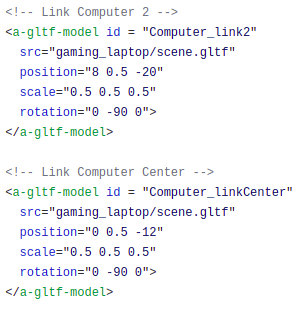
\includegraphics[scale=0.57]{img/paso2_1a.png}
\end{figure}

A continuación, pasaremos a crear los 7 paquetes que queremos intercambiar, de manera que cada uno de ellos empiece desde uno de estos nodos que hemos creado anteriormente y llegue hasta otro diferente. Los crearemos de manera manual, creando las entidades a mano, sin automatizar aun el proceso, y serían los siguientes:

\begin{figure}[h]
\centering
    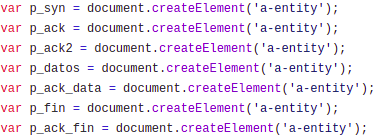
\includegraphics[scale=0.8]{img/paso2_2a.png}
\end{figure}

Y un ejemplo de la composición de uno de ellos sería así:

\begin{figure}[h]
\centering
    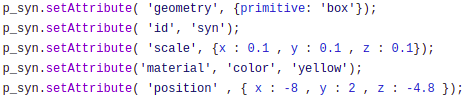
\includegraphics[scale=0.8]{img/paso2_2aa.png}
\end{figure}


Para la conexión de los nodos, crearemos las tuberías transparentes, que crearán la conexión entre los nodos por las que irán los paquetes. Para ello las crearemos de manera manual, y las rotaremos para que nos encajen con las posiciones de los nodos que hemos establecido.



\begin{figure}[h]
\centering
    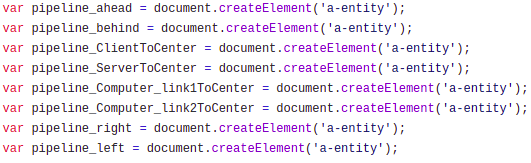
\includegraphics[scale=0.8]{img/paso2_2bb.png}
\end{figure}

\newpage
Y un ejemplo de una de ellas sería la siguiente:

\begin{figure}[h]
\centering
    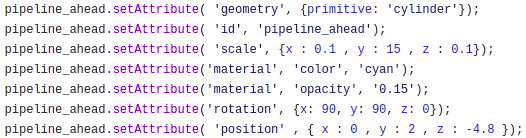
\includegraphics[scale=0.8]{img/paso2_bbb.png}
\end{figure}


Y, para terminar, añadiremos a la escena un botón, el cual nos permitirá iniciar la animación de los paquetes de un ordenador a otro:

\begin{figure}[h]
\centering
    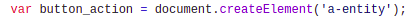
\includegraphics[scale=0.8]{img/boton.png}
\end{figure}

Después añadiremos todos los elementos a la escena y nos pondremos con la creación de los componentes que crearan las animaciones de los paquetes.
El primer componente que he creado es “clicker”, el que gestionara cada click que hagamos en el botón, comprobara que paquete es y lo enviara a la función “moving\_packages” que incorporara la animación a dicho paquete.

\begin{figure}[h]
\centering
    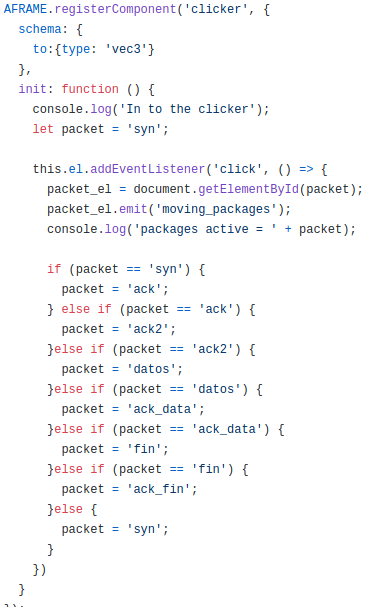
\includegraphics[scale=0.54]{img/clicker.png}
\end{figure}


Y por último añadiremos el componente “move” que incluye la función “moving\_packages”. Esta componente vera que paquete es el que le ha llegado y le añadirá la animación, con la posición destino que le hemos metido manualmente antes, como en este ejemplo:

    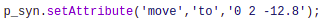
\includegraphics[scale=0.65]{img/paso2_c.png}
, y lo pondrá de color verde.


\begin{figure}[h]
\centering
    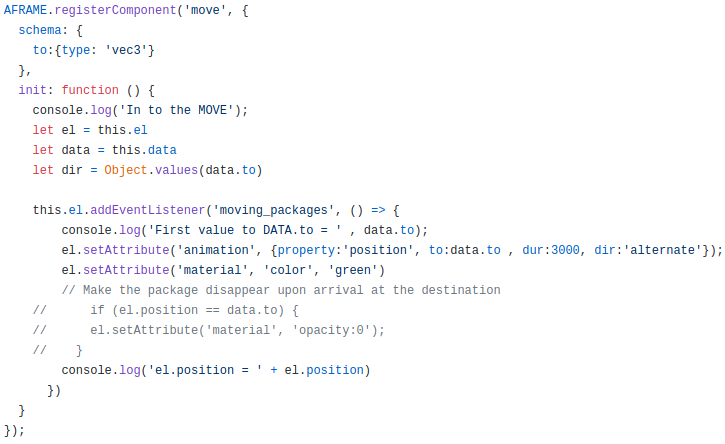
\includegraphics[scale=0.65]{img/move.png}
\end{figure}

Ahora cada vez que se pulsa el botón, el paquete correspondiente cambia de color a verde, y se moverá desde el ordenador origen al destino a través de las tuberías.Y la escena final quedaria así:
\begin{figure}[h]
\centering
    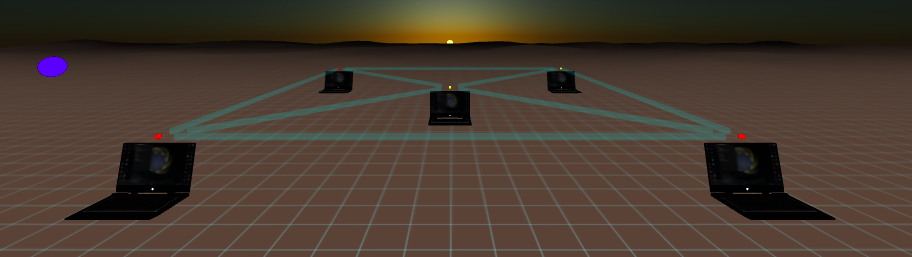
\includegraphics[scale=0.5]{img/escena2_final.png}
\end{figure}

\newpage
En la parte de Wireshark, empezaremos a sacar algunos datos que nos interesan de la captura.
Mediante XMLHttpRequest(), empezaremos a obtener estos datos, realizando al principio una petición GET para ir obteniendo los valores que nos interesen.

\begin{figure}[h]
\centering
    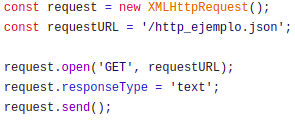
\includegraphics[scale=0.7]{img/GET.png}
\end{figure}

Crearemos un for para recorrer todos los paquetes de la captura y sacar los datos que nos interesan:

\begin{figure}[h]
\centering
    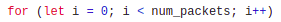
\includegraphics[scale=0.7]{img/for.png}
\end{figure}

Y obtendremos las direcciones IP y Ethernet recorriendo estos campos:

\begin{figure}[h]
\centering
    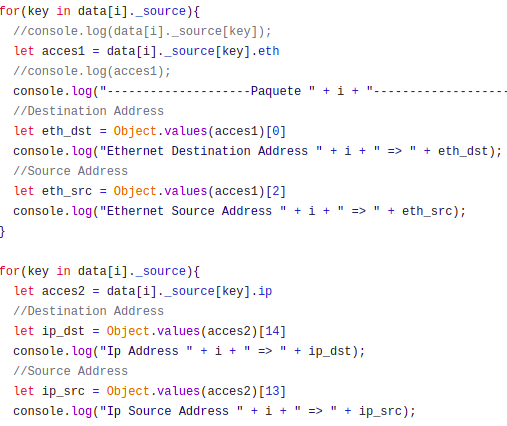
\includegraphics[scale=0.7]{img/datos_json.png}
\end{figure}

\newpage
\subsection{Etapa 3: Componentes}
Ahora comenzaremos con la creación de los componentes para crear de una manera más automatizada los elementos que van a componer nuestra escena.

Empezamos con la construcción del componente para los nodos\footnote{\url{https://alejandroeslo.github.io/TFG/Pruebas/Pasos_seguidos/Demos_componentes/P3_1b.html}}.
. Este componente creará cada uno los nodos con su correspondiente color y posición, que le será enviada al componente como una variable. Aquí podemos ver el componente:

\begin{figure}[h]
\centering
    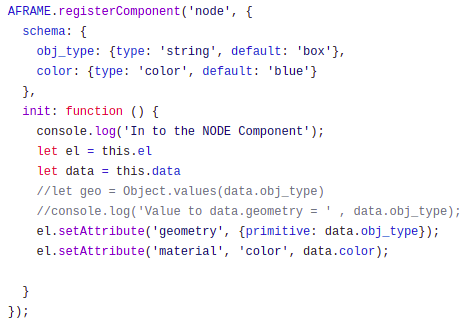
\includegraphics[scale=0.6]{img/node1.png}
\end{figure}

Y crearemos las entidades con los parámetros que nos interesa pasarle luego a nuestro componente “node”:


\begin{figure}[h]
\centering
    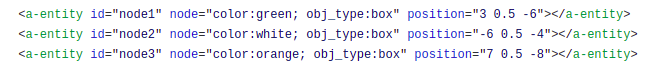
\includegraphics[scale=0.5]{img/node2.png}
\end{figure}

El resultado que obtendremos será el siguiente:

\begin{figure}[h]
\centering
    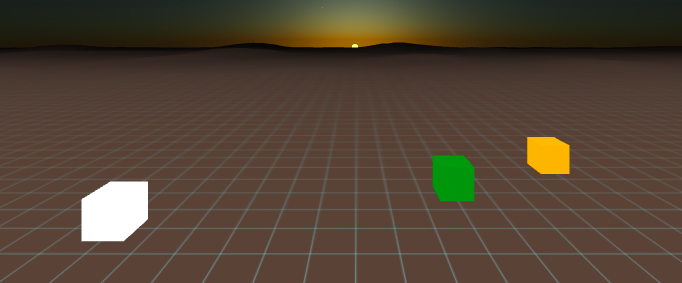
\includegraphics[scale=0.44]{img/componenteNODE.png}
\end{figure}

A continuación crearemos el componente connection, que será el que conectara nuestros nodos mediante tuberías transparentes.

Crearemos las entidades para cada tubería, añadiéndoles el componente connection con los atributos TO y FROM que le introduciremos manualmente de momento.

\begin{figure}[h]
\centering
    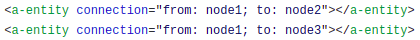
\includegraphics[scale=0.7]{img/entidad_connect.png}
\end{figure}

Más tarde, estos campos los rellenaremos con los datos que extraigamos del archivo JSON.

Ahora vamos a crear el componente connection, cuya función va a ser la de crear las tuberías transparentes que conectan los nodos.

\begin{figure}[h]
\centering
    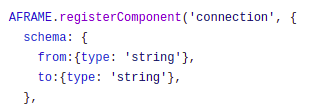
\includegraphics[scale=0.7]{img/comp_conn.png}
\end{figure}

Cogeremos la posición TO y FROM del nodo correspondiente a su Id, y pasaremos estas coordenas a String para luego poderlas pasar como atributo al objeto y crear el elemento.
Aquí podemos ver el ejemplo de las coordenadas FROM:
\begin{figure}[h]
\centering
    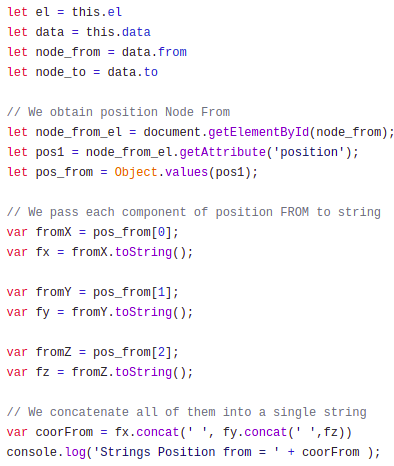
\includegraphics[scale=0.6]{img/datos_from.png}
\end{figure}

Y en esta parte añadiriamos las coordenadas al elemento “tube”,para que nos cree esas conexiones.
\begin{figure}[h]
\centering
    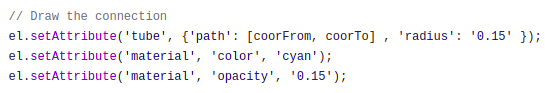
\includegraphics[scale=0.7]{img/puesta_datos.png}
\end{figure}

Y la escena final se vería de esta forma:

\begin{figure}[h]
\centering
    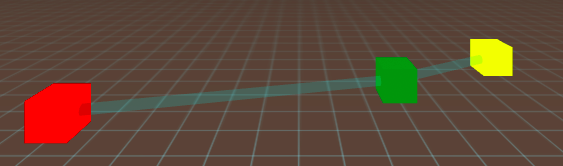
\includegraphics[scale=0.7]{img/componenteCONNECTION.png}
\end{figure}

Por último, crearemos el componente Packet, que será el encargado de ir creando todos los paquetes que vaya encontrando e incluyéndolos en la escena\footnote{\url{https://alejandroeslo.github.io/TFG/Pruebas/Pasos_seguidos/Demos_componentes/P3_3a.html}}.

La entidad creada en este caso estará compuesta por el componente packet, que tendrá los siguientes argumentos:color, duración, nodo from, nodo to, tiempo de comienzo:


\begin{figure}[h]
\centering
    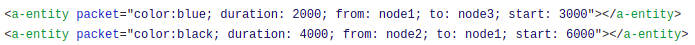
\includegraphics[scale=0.7]{img/entidad_packet.png}
\end{figure}

Y en el componente packet obtendremos también las posiciones TO y FROM de los nodos correspondientes, para saber desde donde va el paquet y hasta donde irá:\\

    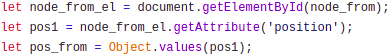
\includegraphics[scale=0.7]{img/pos_packet1.png}

    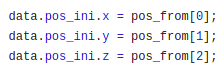
\includegraphics[scale=0.7]{img/pos_packet2.png}
\newpage
Añadiremos todos estos datos como atributo a la entidad y crearemos también la animación que será la que hará que se desplacen los paquetes de un nodo al otro:


\begin{figure}[h]
\centering
    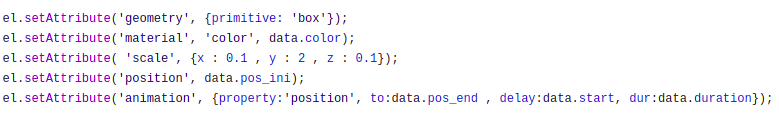
\includegraphics[scale=0.6]{img/atributos_packet.png}
\end{figure}

Y la escena  final sería así:
\begin{figure}[h]
\centering
    \includegraphics[scale=0.7]{img/componentePACKET.png}
\end{figure}

\newpage
\subsection{Etapa 4: Componente Net Simulator}
En este apartado crearemos un nuevo componente, que será el más importante, se trata del componente net-simulator.
Este componente se encargará de sacar todos los datos necesarios para la creación de la escena, y luego irlos pasando a los componentes correspondientes para crear todos los elementos de la escena, nodos, conexiones y paquetes.

Primeramente este componente lo que creará serán todos los nodos que encuentre en la captura, ira iterando por todas las direcciones IP o Ethernet y con ellas creara los nodos de la escena. Aquí comenzaremos creando los nodos de forma lineal para ver como será el funcionamiento, y finalmente acabaremos colocándolos en estructura circular, para que sean visibles todos los nodos.

A continuación creara las conexiones entre estos nodos, solamente creara las conexiones entre los nodos que intercambien paquetes, entre los que no haya ningún intercambio de paquetes no habrá ninguna conexión.

Y por último, creara los paquetes que vengan en la captura y los colocara en el nodo de salida, los cuales se iniciaran la animación después de pulsar el botón.

\subsection{Etapa 5: Manejador botón y puesta de carteles}
Ahora nos ocuparemos de la funcionalidad del botón, para poder controlar la animación correctamente de los paquetes.

Para ello utilizaremos el manejador de tiempos de set interval, para poder iniciar la animación, parar la animación y también reanudar la animación.

Crearemos una función para controlar la animación:
\begin{figure}[h]
\centering
    \includegraphics[scale=0.52]{img/func_run.png}
\end{figure}


Controlaremos el click sobre el botón con un evento que se quede escuchando junto al setinterval y dependiendo del estado en el que se encuentre la variable currentEvent, el botón parara o reanudara la animación:

\begin{figure}[h]
\centering
    \includegraphics[scale=0.65]{img/emit.png}
\end{figure}

Por último en esta etapa, cogeremos las direcciones IP o Ethernet de cada nodo y las colocaremos en un cartel encima de todos los nodos para identificarlos de manera más sencilla.


\begin{figure}[h]
\centering
    \includegraphics[scale=0.7]{img/cartel.png}
\end{figure}

\subsection{Etapa 6: Creación de capas y escena final}

En esta última etapa veremos la creación de las capas en los paquetes y las demos finales.

Para terminar la escena hemos introducido en cada uno de los paquetes, las capas de internet que tienen con los datos más relevantes de cada una de ellas. Estas capas no estarán incluidas en todos los paquetes, cada paquete solo mostrará aquellas capas que traiga incorporadas en la captura realizada, es decir, si un paquete solo tiene capa IP y Ethernet, solamente se mostraran estas capas, en cambio si también tiene TCP y HTTP, mostrara las 4 capas.

Estas capas aparecerán al pinchar sobre cada paquete, y aparecerán en forma de cubos, cada cubo representará una capa, y están ordenadas de menor a mayor importancia, la de abajo será la de Ethernet, luego IP, después TCP y la última HTTP.
\begin{figure}[h]
\centering
    \includegraphics[scale=0.5]{img/capas.png}
\end{figure}

Una vez sean mostradas estas capas, pincharemos sobre la que nos interese para que nos muestre la información que contiene esa capa.

\begin{figure}[h]
\centering
    \includegraphics[scale=0.45]{img/capa_ip.png}
    \includegraphics[scale=0.45]{img/capa_eth.png}
    \includegraphics[scale=0.45]{img/capa_tcp.png}
    \includegraphics[scale=0.44]{img/capa_http4.png}
\end{figure}

\newpage
Y para finalizar, crearemos las escenas finales, donde se verán todos los elementos y funcionalidades finales en una misma escena.

\begin{figure}[h]
\centering
    \includegraphics[scale=0.7]{img/fin1.png}
\end{figure}

\begin{figure}[h]
\centering
    \includegraphics[scale=0.52]{img/din2.png}
\end{figure}

%%%%%%%%%%%%%%%%%%%%%%%%%%%%%%%%%%%%%%%%%%%%%%%%%%%%%%%%%%%%%%%%%%%%%%%%%%%%%%%%
%%%%%%%%%%%%%%%%%%%%%%%%%%%%%%%%%%%%%%%%%%%%%%%%%%%%%%%%%%%%%%%%%%%%%%%%%%%%%%%%
% RESULTADOS %
%%%%%%%%%%%%%%%%%%%%%%%%%%%%%%%%%%%%%%%%%%%%%%%%%%%%%%%%%%%%%%%%%%%%%%%%%%%%%%%%

\cleardoublepage
\chapter{Resultado Final}
\section{Manual de usuario}
\subsection{Usuario de una escena ya constriuida}

En este apartado explicaremos como usar la aplicación en un usuario a nivel alto, es decir, como un usuario con la aplicación ya desplegada en el navegador debería usarla.

Lo primero que deberán de hacer es acceder a una de las demos que hay disponible en mi github\footnote{\url{https://github.com/AlejandroEsLo/TFG}}(demo1\footnote{\url{https://alejandroeslo.github.io/TFG/Demo1_100Packets.html}}, demo2\footnote{\url{https://alejandroeslo.github.io/TFG/Demo2_HTTPPackets.html}}) y abrirla en un navegador.

Una vez nos encontremos en la escena, podremos movernos con las flechas del teclado hacia adelante, hacia atrás y hacia ambos dados. Ayudados del ratón, podremos girar sobre la escena y desplazarnos por toda la escena y acercarnos o alejarnos hacia la parte que nos interese.

Para poner en funcionamiento la animación de los paquetes, deberemos de colocarnos enfrente del botón y pulsarlo con un click del ratón, esto nos permitirá empezar la animación de los paquetes. De esta misma forma, podremos detener los paquetes para analizarlos, y volverlos a poner en marcha cuando queramos de nuevo.
\begin{figure}[h]
\centering
    \includegraphics[scale=0.5]{img/boton_im.png}
\end{figure}

Si ahora queremos analizar los paquetes, lo único que debemos de hacer es clicar sobre un paquete (será más fácil si paramos la animación), y una vez hagamos esto, se nos desplegaran unos subniveles con las capas que contiene cada paquete.

Para ver la información que trae cada capa, volvemos a pinchar en cada uno de estos subniveles y se nos mostrará un cartel con los datos de esa capa.

\begin{figure}[h]
\centering
    \includegraphics[scale=0.45]{img/capa_ip.png}
    \includegraphics[scale=0.45]{img/capa_eth.png}
    \includegraphics[scale=0.45]{img/capa_tcp.png}
    \includegraphics[scale=0.44]{img/capa_http4.png}
\end{figure}

Para cerrar cada subnivel, volvemos a pinchar en el subnivel seleccionado y si queremos salir de la visión de los subniveles, volvemos a pinchar sobre el paquete y se volverán a ocultar.

\subsection{Usuario que construye una escena}

En este apartado veremos como ya un usuario avanzado puede  crear el mismo una escena con los datos que él desee introducir en el programa.

Primeramente realizaremos la captura JSON en Wireshark de la red que nos interese analizar.

Después la exportaremos como un archivo JSON, para ello:
\begin{enumerate}
    \item Pincharemos sobre la pestaña Archivo.
    \item Buscaremos la opción Exportar análisis de paquetes.
    \item Y elegiremos la opción exportar como JSON.
\end{enumerate}
Con esto ya tendríamos exportada nuestra captura para poderla introducir en el programa y crear la escena de dicha captura.

A continuación, lo que hay que hacer es descargarse el repositorio TFG\footnote{\url{https://github.com/AlejandroEsLo/TFG}} de mi github.

Una vez descargado, los archivos que nos interesaran para utilizar seran los siguientes:
\begin{figure}[h]
\centering
    \includegraphics[scale=0.8]{img/archivos.png}
\end{figure}

El primer archivo (100packets\_demo1.json)es la captura JSON que he utilizado yo para la demo, y que sustituiremos por la que queramos usar nosotros. Podemos cambiarle el nombre al archivo si queremos.

El segundo archivo (Demo1\_100Packets.html) es el archivo HTML principal desde donde se cargara el archivo JavaScript con todo el programa completo.


En este archivo podemos ver los parámetros que tiene el componente Net Simulator, y son los siguientes:

\begin{figure}[h]
\centering
    \includegraphics[scale=0.7]{img/parametros.png}
\end{figure}

\begin{itemize}
    \item File: es el parámetro en donde tendremos que introducir el nombre completo de nuestra captura realizada en JSON.
    \item Proto: es el protocolo que nosotros querremos representar en la escena. Este parámetro puede tener dos valores:
    \begin{itemize}
    \item ip : Nos representará todos los nodos de la capa IP.
    \item eth :Nos representará todos los nodos de la capa Ethernet.
    \end{itemize}
\end{itemize}

Estos archivos debene estar en la misma carpeta junto al archivo principal Javascript NetSimulator(NetSimulator.js).

Una vez realizados todos estos pasos, e introducida correctamente la captura en el archivo, procederemos a ejecutar un servidor local con Python para visualizarlo en cualquier navegador.

Para ello, nos situaremos en la carpeta que tengamos los anteriores archivos y abriremos un terminal, y escribiremos la siguiente línea de comandos:

\begin{figure}
\centering
    \includegraphics[scale=0.7]{img/server_python.png}
\end{figure}

\newpage
Después nos dirigimos a cualquier navegador y escribimos la siguiente dirección(teniendo en cuenta el nombre de nuestro archivo si lo hemos cambiado):

\begin{center}
http://localhost:8000/Demo1\_100Packets.html
\end{center}

También podemos ejecutar las demos que hay directamente desde el repositorio de GitHub que antes hacia referencia TFG, y en el README, al pulsar sobre cualquier dirección, te ejecutara la demos para poder visualizarla.

\section{Manual técnico}

En este apartado vamos a ver los detalles de la estructura
del programa y que elementos lo componen.

Los elementos principales del programa son los componentes. Los componentes son módulos de JavaScript que se pueden mezclar, combinar y componer en entidades para crear apariencia, comportamiento y funcionalidad.

Los componentes que componen el simulador son 5: componente poster, componente node, componente connection, componente packet y el componente net-simulator. Este último componente será el más importante, ya que será el que relacionara todos los componentes y creara la escena final.

\subsection{Componente Node}

Este componente será el encargado de crear todos los nodos que sean necesarios en la escena. Tendrá cuatro argumentos de entrada, que le podremos pasar cuando queramos utilizar el componente, que son los siguientes:

\begin{figure}[h]
\centering
    \includegraphics[scale=0.7]{img/arg_comp_node.png}
\end{figure}

\begin{itemize}
    
    \item obj$\_$type: Este argumento nos indicará el tipo de nodo que queremos que nos dibuje en la escena. Puede ser de dos tipos:
    \begin{itemize}
        \item computer : Nos representará los nodos con un gltf de un ordenador(que es el que nos aparece en las demos).
        
        \begin{figure}[h]
            \centering
            \includegraphics[scale=0.7]{img/gltf_comp_node.png}
        \end{figure}
        
        \item Si no ponemos nada, nos dibujara una caja como nodo, con el color que le hayamos indicado en 	la entrada.
        
        \begin{figure}[h]
            \centering
            \includegraphics[scale=0.7]{img/box_comp_node.png}
        \end{figure}
        
    \end{itemize}
    
    \item color: Nos permitirá elegir el color que le queramos poner a cada uno de nuestros nodos.
    
    \item position: En este argumento introduciremos la posición en la que dibujaremos y colocaremos nuestro nodo.
    
    \item id: Será el identificador correspondiente al nodo.
\end{itemize}

En la escena final se verían los nodos de la siguiente forma:
\begin{center}
    \includegraphics[scale=0.58]{img/componenteNode_modelo.png}
\end{center}


\subsection{Componente Connection}

Este componente será el encargado de conectar los nodos creados en el componente anterior mediante tuberías transparentes por las que más adelante pasaran los paquetes de la escena.
Los argumentos que tendremos de entrada en este componente son 2:


\begin{figure}[h]
\centering
    \includegraphics[scale=0.7]{img/arg_comp_connect.png}
\end{figure}

\begin{itemize}
    \item from: Tendremos las coordenadas del nodo from, desde el nodo en el que debe empezar la tubería de la conexión.
    
    \item to: Tendrá las coordenadas del nodo to, desde el nodo en el que acabara la tubería de la conexión.
    
\end{itemize}

La funcionalidad de este componente es recibir las coordenadas “from” y “to” y ponerlas en la tubería que dibujemos para ver desde donde hasta donde va a ir esa tubería.
Para ello cogeremos por ejemplo la variable from que nos llega y con un getElementById del argumento from que recibimos obtenemos el nodo desde donde tiene que salir la tubería, y después con el getAttribute del atributo position del nodo que hemos obtenido anteriormente, obtendremos las coordenadas en las que empezará la tubería.

\begin{figure}[h]
\centering
    \includegraphics[scale=0.7]{img/getPos_comp_connect.png}
\end{figure}

Cogeremos estas coordenadas y las pasamos a string una a una (x,y,z).
\begin{figure}[h]
\centering
    \includegraphics[scale=0.7]{img/xFrom_comp_connect.png}
\end{figure}

A continuación las concatenamos todas para poderla dibujar después.
\begin{center}
    \includegraphics[scale=0.7]{img/concat_comp_connect.png}
\end{center}


Y por último las dibujaremos poniendo los atributos correspondientes usando la primitiva “tube”\footnote{\url{https://www.npmjs.com/package/aframe-extras.tube}}, que nos permitirá dibujar las conexiones.

\begin{center}
    \includegraphics[scale=0.7]{img/draw_comp_connect.png}
\end{center}

En la escena final se verían las conexiones de la siguiente forma:
\begin{center}
    \includegraphics[scale=0.58]{img/componenteCOnnect_modelo.png}
\end{center}


\subsection{Componente Packet}

Este componente tendrá la función de darle forma a los paquetes que contiene la captura, y de controlar el movimiento que estos tendrán al pulsar sobre el botón.

Tendrá varios argumentos de entrada, que le podremos pasar cuando queramos utilizar el componente, y también tenemos otros argumentos que están vacíos y solo los utilizaremos dentro del componente.

Los argumentos de entrada que tenemos son:
\begin{itemize}
    \item id: Será el identificador correspondiente a cada paquete.
    
    \item start: Es el tiempo que tiene que pasar hasta que comience a animarse ese paquete. Se corresponde al time\_relative correspondiente en la captura a cada paquete, que es el tiempo correspondiente a cada paquete.
    
    \item color: El color que pondremos a cada uno de los paquetes, que dependiendo del protocolo más alto que tenga ese paquete, el paquete tendrá un color u otro.
    
    \item duration: Se corresponde al tiempo que transcurre desde que el paquete sale del nodo origen hasta que llega al nodo destino.
    
    \item class: Será la clase a la que pertenece cada paquete.
    
    \item proto: Es el protocolo que hemos elegido al comenzar, para dibujar los nodos con el nivel IP o Ethernet.

    \item LastValue: Es la variable en la que introduciremos el nivel más alto de capa que tenga ese paquete, en nuestro caso, el valor más alto que se puede introducir es HTTP, pero también podrá ser TCP, IP o Ethernet.

    \item info\_from\_ip: Aquí introduciremos la dirección “from” de la capa IP del paquete correspondiente, para luego mostrarlo en el cartel correspondiente a su capa.
    
    \item info\_to\_ip: Aquí introduciremos la dirección “to” de la capa IP del paquete correspondiente, para luego mostrarlo en el cartel correspondiente a su capa.
    
    \item info\_from\_eth: Aquí introduciremos la dirección “from” de la capa Ethernet del paquete correspondiente, para luego mostrarlo en el cartel correspondiente a su capa.
    
    \item info\_to\_eth: Aquí introduciremos la dirección “to” de la capa Ethernet del paquete correspondiente, para luego mostrarlo en el cartel correspondiente a su capa.
    
    \item port\_tcp\_dst: Aquí introduciremos el puerto destino de la capa TCP del paquete correspondiente, para luego mostrarlo en el cartel correspondiente a su capa.
    
    \item port\_tcp\_src: Aquí introduciremos el puerto origen de la capa TCP del paquete correspondiente, para luego mostrarlo en el cartel correspondiente a su capa.

    \item info\_http1: En esta variable introduciremos el campo correspondiente al método HTTP utilizado en la petición o a la respuesta recibida, por ejemplo la petición podría ser un GET, y la respuesta un OK, esta información la usaremos luego para mostrarla en el cartel correspondiente a su capa.
    
    \item info\_http2: En esta variable introduciremos el campo correspondiente a la URL utilizado en la petición HTTP o al código de respuesta recibido, por ejemplo la URL podría ser www.download.html, y el código de respuesta un 200, esta información la usaremos luego para mostrarla en el cartel correspondiente a su capa.

\end{itemize}

Este componente será uno de los más importantes, ya que tendrá varias funcionalidades, las cuales pasaremos a explicar a continuación.

La primera funcionalidad de este componente será la de crear los paquetes primero y situarlos sobre la escena. Esto lo hará cogiendo los datos de las variables anteriormente nombradas, y también obteniendo las posiciones de cada uno de los nodos origen y destino que tendrán que tomar para saber desde qué nodo tendrá que salir el paquete y hasta cuál tendrá que desplazarse. Esto lo haremos igual que en el componente “connection”, utilizando getElementById del argumento para saber las coordenadas de origen y destino del paquete.
Con todos estos datos, crearemos los paquetes ya en la escena:

\begin{figure}[h]
\centering
    \includegraphics[scale=0.7]{img/elem_comp_pack.png}
\end{figure}

A continuación colocaremos también el póster de cada paquete. En este proceso hemos optado por colocar dos pósters, uno por delante y otro girado 180º en las coordenadas x y z, para poder visualizar los pósters tanto si lo queremos ver por delante o por detrás.

\begin{figure}[h]
\centering
    \includegraphics[scale=0.7]{img/postpack1_comp_pack.png}
\end{figure}

\begin{figure}[h]
\centering
    \includegraphics[scale=0.7]{img/postpack2_comp_pack.png}
\end{figure}

Por último, en este componente, controlaremos el tiempo de los paquetes con el setinterval y dependiendo de su estado iremos empezando la animación, congelando los paquetes o reanudando la animación de los paquetes.


\begin{figure}[h]
\centering
    \includegraphics[scale=0.7]{img/currevnt_comp_pack.png}
\end{figure}

\newpage
Podemos ver como, cada vez que hacemos click en el botón, cambiara el estado de nuestra variable “currentEvent”, y dependiendo de ese estado, la funcionalidad de los paquetes será distinta.

Después crearemos dos variables(“active” y “view\_info”), que utilizaremos para saber cuando mostrar los carteles de cada paquete o cuando mostrar las capas de los paquetes. Para ello crearemos otro evento y dependiendo del estado de estas variables realizaremos una tarea u otra.

El primero de los estados que vamos a ver es cuando las dos variables estén activas (“on”):

\begin{figure}[h]
\centering
    \includegraphics[scale=0.7]{img/eventlist1_comp_pack.png}
\end{figure}

En este estado, querremos que se vean tanto las capas como los carteles, por lo tanto los pondremos en visible, y añadiremos los textos correspondientes a cada uno de las capas de los paquetes. Aquí podemos ver un ejemplo del caso de la capa IP:

\begin{figure}[h]

    \includegraphics[scale=0.45]{img/ejemplo1ip_comp_pack.png}
\end{figure}
Esto lo haremos para cada una de las capas que tengamos , pero con su correspondiente información.

El segundo estado que nos encontraremos será cuando “active” esté en “on” y “view\_info” en “off”:

\begin{figure}[h]
\centering
    \includegraphics[scale=0.7]{img/eventlist2_comp_pack.png}
\end{figure}

En este estado, querremos que se vean las capas del paquete, pero no los carteles porque llegaran sin información, ya que no tendrán en este caso. Aquí podemos ver un ejemplo del caso de la capa IP:

\begin{figure}[h]
\centering
    \includegraphics[scale=0.6]{img/ejemplo2ip_comp_pack.png}
\end{figure}

Esto lo haremos para cada una de las capas que tengamos , pero con su correspondiente información.

El siguiente estado que nos encontraremos será cuando “active” esté en “off” y “view\_info” en “off”:

\begin{figure}[h]
\centering
    \includegraphics[scale=0.7]{img/eventlist3_comp_pack.png}
\end{figure}
\newpage
En este estado, lo que queremos es que no nos muestre ni la capa y no los carteles, por ello pondremos el atributo “visible” en “false”. Aquí podemos ver un ejemplo del caso de la capa IP:

\begin{figure}[h]
\centering
    \includegraphics[scale=0.8]{img/ejemplo3ip_comp_pack.png}
\end{figure}

Esto lo haremos para cada una de las capas que tengamos , pero con su correspondiente información.

El último estado que nos encontraremos será cuando “active” esté en “off” y “view\_info” en “on”:

\begin{center}
    \includegraphics[scale=0.7]{img/eventlist4_comp_pack.png}
\end{center}

En este estado, como en el anterior, lo que queremos es que no nos muestre ni la capa y no los carteles, por ello pondremos el atributo “visible” en “false”. Aquí podemos ver un ejemplo del caso de la capa IP:

\begin{figure}[h]
\centering
    \includegraphics[scale=0.8]{img/ejemplo4ip_comp_pack.png}
\end{figure}

Esto lo haremos para cada una de las capas que tengamos , pero con su correspondiente información.

En la escena final se verían los paquetes de la siguiente forma:
\begin{center}
    \includegraphics[scale=0.58]{img/componentePacket_modelo.png}
\end{center}

\subsection{Componente Poster}

Este componente será el encargado de crear los carteles o póster que se ponen en cada una de las capas o encima de los nodos que sean necesarios en la escena. Tendrá tres argumentos de entrada, que le podremos pasar cuando queramos utilizar el componente, que son los siguientes:

\begin{figure}[h]
\centering
    \includegraphics[scale=0.7]{img/arg_comp_poster.png}
\end{figure}

\begin{itemize}
    
    \item color: Este argumento nos indicará el color de fondo que tendrá el póster.
    
    \item postion: Este argumento nos indicará la posición en la que ira colocado el póster.
    
    \item text: Este argumento nos indicará el texto que pondremos dentro del póster correspondiente.
 
\end{itemize}

Después procederemos a dibujarlos poniendo los atributos correspondientes usando la primitiva “plane”, que nos permitirá dibujar estos carteles.

\begin{center}
    \includegraphics[scale=0.7]{img/atrib_comp_poster.png}
\end{center}

\newpage
\subsection{Componente Net-simulator}


Este componente será el más importante de todo el programa, ya que su función será la de unir todos los componentes anteriormente mencionados y enviarles todos los datos necesarios para después poder dibujar cada elemento en su correspondiente posición.

Tiene dos argumentos de entrada, que son los siguientes:

\begin{center}
    \includegraphics[scale=0.7]{img/arg_comp_netsim.png}
\end{center}

\begin{itemize}
    \item file: Será el archivo JSON qué queramos analizar en nuestro programa. EN nuestra demo, utilizamos por ejemplo este archivo (file: 100packets\_demo1.json).

    \item proto: Será el protocolo que utilizaremos para dibujar la capa de los nodos. Puede ser ip o eth, dependiendo la variable que elijamos, nos dibujara los nodos con las direcciones Ethernet o los nodos con las direcciones IP.

\end{itemize}


Este componente de lo primero que se va a encargar será de ir sacando los datos necesarios de la captura que le introduzcamos en formato JSON. Para ello lo que haremos será crear un XMLHttpRequest() e iniciarlo con un GET, después iremos sacando los datos que veamos que nos interesa del archivo JSON.

\begin{center}
    \includegraphics[scale=0.7]{img/get_comp_netsim.png}
\end{center}

Primero sacaremos el time relative de cada paquete, que será el que utilizaremos par ver cuando tiene que salir cada uno de los paquetes del nodo origen.
Lo multiplicaremos por 5000 ms para que tenga un tiempo que podamos apreciar en la animación de manera correcta.

\begin{center}
    \includegraphics[scale=0.7]{img/timerelat_comp_netsim.png}
\end{center}
\newpage
Después nos centraremos en sacar los direcciones origen y destino de cada uno de los paquetes, tanto las direcciones Ethernet:

\begin{center}
    \includegraphics[scale=0.7]{img/eth_comp_netsim.png}
\end{center}

como las direcciones IP:

\begin{center}
    \includegraphics[scale=0.7]{img/ip_comp_netsim.png}
\end{center}

Ahora pasaremos a ir creando todos los elementos que queremos incluir en la escena. Primeramente comenzaremos por colocar los nodos de la escena.

Comenzaremos creando una pequeña condición que dependerá del argumento que hayamos puesto al principio en el componente Net-simulator, y dependiendo del protocolo de entrada que hayamos metido, cogeremos el array con los datos de la capa Ethernet o la capa IP.


\begin{center}
    \includegraphics[scale=0.7]{img/condproto_comp_netsim.png}
\end{center}

Después iniciaremos unas variables que nos servirán para ir colocando tanto los nodos como los póster de cada uno de ellos. Tendremos una variable para la posición inicial de los nodos(node\_pos), otra variable con la posición inicial de los póster de su correspondiente nodo (poster\_pos), y luego otras dos variables que usaremos para colocar los nodos en una red tipo circular e iremos aumentando estas variables según vayamos introduciendo más nodos (variables increase y angle).

\begin{center}
    \includegraphics[scale=0.7]{img/varini_comp_netsim.png}
\end{center}


Ahora crearemos un “for” que recorrerá todo el array de nodos que hayamos elegido.

\begin{center}
    \includegraphics[scale=0.7]{img/fornode_comp_netsim.png}
\end{center}

Cada vez que pasemos por este bucle, cambiaremos la posición X y Z del nodo para formar la red circular como anteriormente habíamos comentado.

\begin{center}
    \includegraphics[scale=0.7]{img/posXZ_comp_netsim.png}
\end{center}

Incrementaremos el ángulo también para colocar los nodos correctamente.

\begin{center}
    \includegraphics[scale=0.7]{img/angleincr_comp_netsim.png}
\end{center}


Después añadiremos los atributos necesarios al componente “node” para que nos cree todos los nodos.


\begin{center}
    \includegraphics[scale=0.7]{img/node1_comp_netsim.png}
\end{center}


\begin{center}
    \includegraphics[scale=0.7]{img/node2_comp_netsim.png}
\end{center}

Y finalmente dibujaremos el nodo en la escena final.

\begin{center}
    \includegraphics[scale=0.7]{img/escenanode_comp_netsim.png}
\end{center}

Para los carteles de los nodos, la única posición que cambiaremos será la posición Y para que se pongan encima del nodo final.

\begin{center}
    \includegraphics[scale=0.7]{img/posterY_comp_netsim.png}
\end{center}

\newpage
Añadiremos los atributos correspondientes de cada cartel.

\begin{center}
    \includegraphics[scale=0.7]{img/atribposter_comp_netsim.png}
\end{center}

Y finalmente colocaremos tanto el póster delantero como el trasero ,para verlo por los dos lados en la escena final.

\begin{center}
    \includegraphics[scale=0.7]{img/escenapost_comp_netsim.png}
\end{center}

Ahora pasaremos a dibujar las tuberías de conexión entre los nodos. Para ello, primeramente crearemos también un pequeño “if” en el cual elegiremos un array u otro dependiendo del protocolo de entrada como anteriormente hemos visto.

\begin{center}
    \includegraphics[scale=0.7]{img/ifINIconn_comp_netsim.png}
\end{center}

Después crearemos un “for” que recorrerá todo este array para coger los datos necesarios:

\begin{center}
    \includegraphics[scale=0.7]{img/forConne_comp_netsim.png}
\end{center}

Después añadiremos los atributos necesarios al componente “connection” para que nos cree estas tuberías.

\begin{center}
    \includegraphics[scale=0.7]{img/atribConn_comp_netsim.png}
\end{center}

Y por último añadiremos la tubería a la escena final.

\begin{center}
    \includegraphics[scale=0.7]{img/escenaConn_comp_netsim.png}
\end{center}

\newpage
Finalmente crearemos los paquetes y los iremos añadiendo a la escena final.
\newline
Primeramente comprobaremos el protocolo elegido para la escena, como en los casos anteriores y dependiendo de eso elegiremos unos arrays u otros para obtener los valores necesarios.

\begin{center}
    \includegraphics[scale=0.7]{img/ifPack_comp_netsim.png}
\end{center}

A continuación iremos sacando los datos de cada capa, los cuales utilizaremos para los carteles de cada paquete. Sacaremos los datos de la capa Ethernet, IP, TCP y HTTP. En este caso veremos el ejemplo de los datos de la capa IP:

\begin{center}
    \includegraphics[scale=0.7]{img/ipdatacartel_comp_netsim.png}
\end{center}

Por último veremos cuál es el protocolo más alto que contiene cada paquete, y dependiendo de eso, el paquete lo pintaremos de un color u otro:

\begin{center}
    \includegraphics[scale=0.7]{img/protoColorFInal_comp_netsim.png}
\end{center}

Para acabar enviaremos todos estos valores obtenidos al componente “packet”, para que con ellos elabore todos los paquetes correspondientes:

\begin{center}
    \includegraphics[scale=0.7]{img/atribPAckt_comp_netsim.png}
\end{center}

Y después lo añadiremos todo a la escena:

\begin{center}
    \includegraphics[scale=0.7]{img/escenaPack_comp_netsim.png}
\end{center}
    

%%%%%%%%%%%%%%%%%%%%%%%%%%%%%%%%%%%%%%%%%%%%%%%%%%%%%%%%%%%%%%%%%%%%%%%%%%%%%%%%
%%%%%%%%%%%%%%%%%%%%%%%%%%%%%%%%%%%%%%%%%%%%%%%%%%%%%%%%%%%%%%%%%%%%%%%%%%%%%%%%
% CONCLUSIONES %
%%%%%%%%%%%%%%%%%%%%%%%%%%%%%%%%%%%%%%%%%%%%%%%%%%%%%%%%%%%%%%%%%%%%%%%%%%%%%%%%

\cleardoublepage
\chapter{Conclusiones}
\label{chap:conclusiones}

\section{Consecución de objetivos}
\label{sec:consecucion-objetivos}

Esta sección es la sección espejo de las dos primeras del capítulo de objetivos, donde se planteaba el objetivo general y se elaboraban los específicos.

Hemos logrado superar el objetivo general que era construir un simulador de redes de comunicación basado
en Realidad Virtual, el cual podrá visualizarse en cualquier dispositivo que tenga navegador
web y en dispositivos de realidad virtual. Sin duda, este objetivo esta más que superado, ya que finalmente hemos podido construir este simulador, que es capaz de leer una captura de trazas de red de Wireshark, exportándolos en un JSON, y con los datos obtenidos crear una escena en realidad virtual en la que se dibujan todos los elementos que la componen.

Centrándonos un poco más en los objetivos específicos, se han logrado concluir con éxito todos los objetivos previstos. Primeramente queríamos que el programa se pudiera visualizar de manera sencilla en cualquier navegador y sin tener que instalar ningún programa externo, y además de ello, poder verlo en cualquier dispositivo móvil o dispositivos de realidad virtual, esto lo hemos conseguido gracias a que hemos ido almacenando todo el proyecto en un repositorio de GitHub y con una simple dirección URL, puedes acceder a cualquiera de las demos que se encuentran alojadas en ese repositorio.

Otro gran objetivo era el de familiarizarnos y entender el framework de A-Frame. Esta librería es fundamental en nuestro proyecto, por lo que desde el principio nos hemos metido en profundidad con toda su documentación y ejemplos que hemos ido creando para ir entendiendo mejor esta tecnología y poder progresar correctamente en nuestro proyecto.


Hemos sido capaces de dar animación a nuestros paquetes, que era otro de los objetivos específicos que teníamos por hacer. Mediante un botón que se encuentra en la escena, somos capaces de comenzar la animación, congelar la animación en cualquier momento y reanudarla nuevamente cuando deseemos.
Esta función nos facilitará la inspección de los paquetes, porque podremos congelar el paquete que queramos y pinchar sobre el paquete que nos interese, en el que se nos desplegaran las capas que lleva el paquete y poder ver la información que transporta en cada una de ellas. Pueden traer información de los protocolos que hemos incluido en este proyecto que son:Ethernet , IP , TCP y HTTP.


\section{Aplicación de lo aprendido}
\label{sec:aplicacion}

A lo largo del grado he podido aprender conocimientos de muchas ramas diferentes. En este caso nos centraremos sobre todo en la rama de programación y conocimientos de protocolos de internet.

Empezamos el grado con la asignatura de Informática I, en la cual te introducen de una manera sencilla, en el mundo de la programación y te enseñan los conceptos básicos y fundamentales para ello.

Después vamos avanzando en otras asignaturas como por ejemplo Informática II, Gráficos y Visualización en 3D, Laboratorio de Tecnologías Audiovisuales en la Web, Construcción de Servicios y Aplicaciones Audiovisuales en Internet, en las cuales ya nos vamos centrando en diferentes lenguajes de programación y en programas y conceptos más complejos, con los que iremos ampliando nuestros conocimientos y mejorando nuestras habilidades como programadores. En estas asignaturas hemos aprendido a usar Python, JavaScript y HTML, estas dos últimas son en las que se basan nuestro simulador.

Por otro lado hemos visto también en asignaturas como Protocolos para la Transmisión de Audio y Video en Internet, Arquitectura de Internet y en Sistemas Telemáticos para Medios Audiovisuales, todo lo relacionado con las redes de comunicaciones, fundamentos de estas comunicaciones, protocolos de red, infraestructuras de red, ejemplos y utilización de estas redes... y de este conjunto de asignaturas hemos podido obtener información sobre todo de los protocolos y del comportamiento de los paquetes y las redes, para poderlo aplicar de manera correcta en nuestro simulador.


\section{Lecciones aprendidas}
\label{sec:lecciones_aprendidas}

A lo largo del Trabajo Fin de Grado he podido ampliar mis conocimientos en los siguientes campos:

\begin{enumerate}
  \item Aprendizaje profundo del framework de A-Frame. Gracias a este framework he podido aprender a crear escenas en 3D, colocar elementos en la escena con diferentes comportamientos y formas, darles animación a elementos de la escena, manejo de luces y cámaras. También he aprendido conceptos de ThreeJS (una de las librerías en la que se basa A-Frame).
  
  \item Crear y manejar componentes enteros dentro de mi programa y poder utilizarlos dentro de otros componentes.
  
  \item Importación de modelos 3D para incorporarlos en la escena y hacer que sean un elemento más en ella.
  
  \item Manejo de eventos y modificación de elementos a tiempo real mediante el uso de JavaScript.
  
  \item He aprendido a manipular el DOM haciendo uso de las herramientas del DOM mediante JavaScript.
  
  \item He tenido la oportunidad de realizar pruebas con las gafas de realidad virtual, en las que he podido aprender como utilizarlas y que se puede llegar a hacer y ver en ellas.
  
  \item Uso de LaTeX para la edición de textos científicos y técnicos.
  
\end{enumerate}

\newpage
\section{Trabajos futuros}
\label{sec:trabajos_futuros}

En este apartado podemos ver reflejadas las posibles mejoras o implementaciones que se podrían llegar a introducir en un futuro en este proyecto:

\begin{itemize}
    \item Primeramente se podría mejorar el aspecto en general de la escena, tanto iluminación como el fondo, los paquetes o elementos que se ven en la escena.
    
    \item Se podrían incluir más protocolos de los introducidos por el momento en el proyecto, y con ello conseguir que se pueda obtener otro tipo de información en los paquetes.
    
    \item Podría crearse una barra de tiempo(estilo YouTube) para ver en que momento de la animación te encuentras, saber cuanto te queda para finalizar la animación, o poder deslizarte sobre ella y avanzar o retroceder la animación.
    
    \item Se podría crear un archivo JSON de una red por ejemplo local, con los elementos que la componen y sus direcciones y asignarle un modelo 3D de un elemento diferente(switch, ordenador, móvil...), y con esto podríamos obtener una escena más exacta con los elementos que la componen. Es decir, si el programa detecta una dirección que corresponde a un switch, te dibuje un switch como nodo en vez de un ordenador, o cualquier elemento que queramos incorporarle.
\end{itemize}


%%%%%%%%%%%%%%%%%%%%%%%%%%%%%%%%%%%%%%%%%%%%%%%%%%%%%%%%%%%%%%%%%%%%%%%%%%%%%%%%
%%%%%%%%%%%%%%%%%%%%%%%%%%%%%%%%%%%%%%%%%%%%%%%%%%%%%%%%%%%%%%%%%%%%%%%%%%%%%%%%
% BIBLIOGRAFIA %
%%%%%%%%%%%%%%%%%%%%%%%%%%%%%%%%%%%%%%%%%%%%%%%%%%%%%%%%%%%%%%%%%%%%%%%%%%%%%%%%

\cleardoublepage

% Las siguientes dos instrucciones es todo lo que necesitas
% para incluir las citas en la memoria
\bibliographystyle{abbrv}
\bibliography{memoria}  % memoria.bib es el nombre del fichero que contiene
% las referencias bibliográficas. Abre ese fichero y mira el formato que tiene,
% que se conoce como BibTeX. Hay muchos sitios que exportan referencias en
% formato BibTeX. Prueba a buscar en http://scholar.google.com por referencias
% y verás que lo puedes hacer de manera sencilla.
% Más información: 
% http://texblog.org/2014/04/22/using-google-scholar-to-download-bibtex-citations/     


\nocite{A-Frame}

\nocite{A-Framewidgets}

\nocite{A-Framegui}

\nocite{TimeInterval}

\nocite{Timer}

\nocite{Aframe-playground}

\nocite{overleaf}

\nocite{event}

\nocite{}

\end{document}
